\chapter{\matricesTitle}
\label{Matrices}

Matrices are a powerful tool for calculations involving linear transformations.
It is important to understand how to find the matrix of a linear transformation 
and the properties of matrices.

\section{Linear Transformations and Matrices}

Ordered, finite-dimensional, bases for  vector spaces allows us to express linear operators as matrices.
%We represent vectors from $\Re^n$ as matrices with one column, so lets begin there.

\subsection{Basis Notation}
\hypertarget{Basis notation}{~}

\noindent
A basis allows us to efficiently label arbitrary vectors in terms of column vectors. Here is an  example.
\begin{example}
Let \[V=\left\{\begin{pmatrix}a&b\\c&d\end{pmatrix}\middle| \,a,b,c,d\in {\mathbb R}\right\}\] be the vector space of $2\times 2$ real matrices,
with addition and scalar multiplication defined componentwise. 
One choice of basis is the ordered set (or list) of matrices
\[B=\left(\begin{pmatrix}1&0\\0&0\end{pmatrix},\begin{pmatrix}0&1\\0&0\end{pmatrix},\begin{pmatrix}0&0\\ 1&0\end{pmatrix},\begin{pmatrix}0&0\\ 0&1\end{pmatrix}\right)=:(e_1^1,e_2^1,e^2_1,e^2_2)\, .\] 
Given a particular vector and a basis, your job is to write that vector as a sum of multiples of basis elements. Here
an arbitrary vector $v\in V$ is just a matrix, so we write
\begin{eqnarray*}
v\ =\ \begin{pmatrix}a&b\\c&d\end{pmatrix}&=&\quad\!\! \begin{pmatrix}a&0\\0&0\end{pmatrix}+\begin{pmatrix}0&b\\0&0\end{pmatrix}+\begin{pmatrix}0&0\\ c&0\end{pmatrix}+\begin{pmatrix}0&0\\0&d\end{pmatrix}\\[1mm]
&=&a\begin{pmatrix}1&0\\0&0\end{pmatrix}+b\begin{pmatrix}0&1\\0&0\end{pmatrix}+c\begin{pmatrix}0&0\\ 1&0\end{pmatrix}
+d\begin{pmatrix}0&0\\0&1\end{pmatrix}\\[1mm]
&=&a\,  e^1_1+b \, e^1_2+c \, e^2_1+d \, e^2_2\, .
\end{eqnarray*}
The coefficients $(a,b,c,d)$ of the basis vectors $(e^1_1,e^1_2,e^2_1,e^2_2)$ encode the information of which matrix the vector $v$ is.
We store them in column vector by writing
\[
v=a \, e^1_1+b \, e^1_2+c\,  e^2_1+d \, e^2_2=: (e^1_1,e^1_2,e^2_1,e^2_2)\colvec{a\\b\\c\\d}=:\colvec{a \\ b\\c\\d}_B\, .
\]
The 4-vector $\colvec{a\\b\\c\\d} \in \mathbb{R}^4$ encodes the vector $\begin{pmatrix}a&b\\c&d\end{pmatrix}\in V$ but is NOT equal to it! \\(After all, $v$ is a matrix so could not equal a column vector.) Both notations on the right hand side of the above equation really stand for the vector obtained by multiplying the coefficients stored in the column vector by the corresponding basis element and then summing over them.
\end{example}
 
Next, lets consider a tautological example showing how to label column vectors in terms of column vectors:

\begin{example} (Standard Basis of $\Re^2$)\index{Standard basis!for ${\mathbb R}^2$}\\
The vectors 
\[
e_1=\colvec{1\\0},~~~
e_2=\colvec{0\\1}
\]
are called the standard basis vectors of $\Re^2=\Re^{\{1,2\}}$. 
Their description as functions of~$\{1,2\}$ are 
\begin{displaymath}
   e_1 (k)= \left\{
     \begin{array}{lr}
       1 & {\rm ~if~} k=1\\
       0 & {\rm ~if~} k=2
     \end{array}
   \right. \, ,~~
   e_2 (k)= \left\{
     \begin{array}{ll}
       0 & {\rm ~if~} k=1\\
       1 & {\rm ~if~} k=2\, .
     \end{array}
   \right.
\end{displaymath} 
It is  natural to assign these  the order: $e_1$ is first and $e_2$ is second.
An arbitrary vector~$v$ of $\Re^2$ can be written as  
\[
v=\colvec{x\\y}=x e_1+ ye_2 .
\]
To emphasize that we are using the standard basis we define the list (or ordered set) \[E=(e_1,e_2)\, ,\] and write 
\[
\colvec{x\\y}_E:=(e_1,e_2)\colvec{x\\y}:=x e_1+ ye_2=v .
\]
You should read this equation by saying:
\begin{quote}
``The column vector of the vector $v$ in the basis $E$ is $\colvec{x\\y}$.''
\end{quote}

Again, the first notation of a column vector with a subscript~$E$ refers to the vector obtained by multiplying each basis vector
by the corresponding scalar listed in the column and then  summing these, {\itshape i.e.} $xe_1+y e_2$. 
The second notation denotes exactly the same thing but we first list the basis elements and then the column vector; a useful trick
because this can be read in the same way as matrix multiplication of a row vector times a column vector--except that the entries of the row vector are themselves vectors! 
\end{example}

You should already try to write down the standard basis vectors for $\Re^n$ for other values of $n$ and express an arbitrary vector in $\Re^n$  in terms of them.%webwork problem? 

The last example probably seems pedantic because column vectors are already just ordered lists of numbers and the basis notation 
has simply allowed us to ``re-express'' these as lists of numbers. Of course, this objection does not apply to more complicated vector spaces like our first matrix example. Moreover, as we saw \hypertarget{nonstandard r2 basis}{earlier}, there are infinitely many other pairs of vectors in $\Re^2$ that form a basis.

\begin{example}(A Non-Standard Basis of $\Re^2=\Re^{\{1,2\}}$)\\
\[
b=\colvec{1\\1}\, ,\quad \beta=\colvec{1\\-1}.
\]
As functions of $\{1,2\}$ they read
\begin{displaymath}
   b (k)= \left\{
     \begin{array}{lr}
       1 & {\rm ~if~} k=1\\
       1 & {\rm ~if~} k=2
     \end{array}
   \right. \, ,~~
   \beta (k)= \left\{
     \begin{array}{rl}
       1 & {\rm ~if~} k=1\\
       -1 & {\rm ~if~} k=2\, .
     \end{array}
   \right.
\end{displaymath} 

Notice something important: there is no reason to say that $\beta$ comes before $b$ or vice versa. That is, there is no {\itshape a priori} reason to give these basis elements one order or the other. 
However, it will be necessary to give the basis elements an order if we want to use them to encode other vectors.  We choose one arbitrarily; let \[B=(b,\beta)\] be the ordered basis. Note that for an unordered set we use the $\{\}$ parentheses while for lists or ordered sets we use $()$. 

As before we define 
\[
\colvec{x\\y}_B :=(b,\beta)\colvec{x \\ y}:= xb+ y \beta\, . 
\]
You might think that the numbers $x$ and $y$ denote exactly the same vector as in the previous example. However, they do not. Inserting
the actual vectors that $b$ and $\beta$ represent we have
\[
xb+ y \beta=x\colvec{1\\1}+y\colvec{1\\-1}=\colvec{x+y\\x-y}\, .
\]
Thus, to contrast, we have
\[
\colvec{x\\y}_B=\colvec{x+y\\x-y} \mbox{ and } \colvec{x\\y}_E=\colvec{x\\y}
\]
Only in the standard basis $E$ does the column vector of $v$ agree with the column vector that $v$ actually is!

%This equation shows how a pair of numbers in ordered basis $B$ gives a pair of numbers in the standard basis $E$. The stacks of numbers we have dealt with in the past were always specifying vectors in the standard basis. 

%The other order for the basis, $B'=(\beta,b)$ yields
%\[
%\colvec{x\\y}_B' := x\beta+ y b =x\colvec{1\\-1}+y \colvec{1\\1}=\colvec{x-y\\x+y}_E.
%\]
%Again, order matters. 
\end{example}

Based on the above example, you might think that our aim would be to find the ``standard basis'' for any problem. 
In fact, this is far from the truth. Notice, for example that the vector \[v=\colvec{1\\1}=e_1+e_2=b\] written in the standard basis~$E$ is just
\[
v=\colvec{1\\1}_E\, ,
\]
which was easy to calculate. But in the basis~$B$ we find
\[
v=\colvec{1\\0}_B\, ,
\]
which is actually a simpler column vector!
The fact that there are many bases for any given vector space allows us to choose a basis in which our computation is easiest. 
In any case, the standard basis only makes sense for $\Re^n$. Suppose your vector space was the set of solutions to a differential equation--what would a standard basis then be?



\begin{example} (A Basis For a Hyperplane)\\
Lets again consider the hyperplane
\[
V=\left\{  c_1\colvec{1\\1\\0} +c_2\colvec{0\\1\\1} \middle| c_1,c_2\in \Re \right\} 
\]
One possible choice of ordered basis is 
\[b_1=\colvec{1\\1\\0},~~~b_2=\colvec{0\\1\\1}, ~~~
B=(b_1,b_2).
\]
With this choice
\[
\colvec{x\\y}_B := xb_1+ y b_2 
=x\colvec{1\\1\\0}+y \colvec{0\\1\\1}=\ccolvec{x\\x+y\\y}_E.
\]
With the other choice of order $B'=(b_2, b_1)$ 
\[
\colvec{x\\y}_{\!B'} := xb_2+ y b_1 
=x\colvec{0\\1\\1}+y \colvec{1\\1\\0}=\ccolvec{y\\x+y\\x}_E.
\]
We see that the  order of basis elements matters. 
\end{example}

Finding the column vector of a given vector in a given basis usually amounts to a linear systems problem:

\begin{example} (Pauli Matrices)\\
Let \[V=\left\{\begin{pmatrix}z&u\\v&-z\end{pmatrix}\middle| z,u,v\in{\mathbb C}\right\}\]\
be the vector space of \hyperlink{TRACE}{trace}-free complex-valued matrices (over~${\mathbb C}$) with basis
\[
B=(\sigma_x,\sigma_y,\sigma_z)\, ,
\] where
\[
\sigma_x=\begin{pmatrix}0&1\\1&0\end{pmatrix}\, ,\quad
\sigma_y=\begin{pmatrix}0&-i\\i&0\end{pmatrix}\, ,\quad
\sigma_z=\begin{pmatrix}1&0\\0&-1\end{pmatrix}\, .
\]
These three matrices are the famous {\itshape Pauli matrices}\index{Pauli Matrices}; they are used to describe electrons in quantum theory, or qubits in quantum computation.
Let 
\[
v=\begin{pmatrix}
-2+i&1+i\\3-i&2-i
\end{pmatrix}\, .
\]
Find the column vector of $v$ in the basis~$B$.

For this we must solve the equation
\[
\begin{pmatrix}
-2+i&1+i\\3-i&2-i
\end{pmatrix}
=\alpha^x \begin{pmatrix}0&1\\1&0\end{pmatrix}+\alpha^y
\begin{pmatrix}0&-i\\i&0\end{pmatrix}+\alpha^z
\begin{pmatrix}1&0\\0&-1\end{pmatrix}\, .
\]
This gives four equations, {\itshape i.e.} a linear systems problem, for the $\alpha$'s
\[
\left\{
\begin{array}{rrrrr}
\alpha^x&\!\!-\ i\alpha^y&&=&1+i\\
\alpha^x&\!\!+\ i\alpha^y&&=&3-i\\
&&\alpha^z&=&-2+i\\
&&-\alpha^z&=&2-i\\
\end{array}
\right.
\]
with solution
\[
\alpha^x=2\, ,\quad \alpha^y=2-2i\, ,\quad \alpha^z=-2+i\, .
\]
Thus
\[
v=\begin{pmatrix}
-2+i&1+i\\3-i&2-i
\end{pmatrix}=\ccolvec{2\\\ 2-i\\\!\!-2+i }_B\, .
\]
\end{example}

To summarize, the {\itshape column vector 
of a vector}\index{Column vector! of a vector} $v$ in an ordered basis $B=(b_1,b_2,\ldots,b_n)$,
\[\ccolvec{\alpha^1\\\alpha^2\\\vdots\\\alpha^n}\, ,\] is defined by solving the linear systems problem
\[
v=\alpha^1 b_1 + \alpha^2b_2 +\cdots + \alpha^n b_n = \sum_{i=1}^n \alpha^i b_i\, .
\]
The numbers $(\alpha^1,\alpha^2,\ldots,\alpha^n)$ are called the {\itshape components of the vector}\index{Components of a vector}~$v$.
Two useful shorthand notations for this are
\[
v=\ccolvec{\alpha^1\\\alpha^2\\\vdots\\\alpha^n}_B = (b_1,b_2,\ldots,b_n)\ccolvec{\alpha^1\\\alpha^2\\\vdots\\\alpha^n}\, .
\]

\subsection{From Linear Operators to Matrices}

Chapter~\ref{sec:linearTransformation} showed that linear functions are very special kinds of functions; 
they are fully specified by their values on any basis for their domain. 
A matrix  records how a linear operator maps an element of the basis to a sum of multiples in the target space basis.

More carefully, if $L$ is a linear operator from $V$ to $W$ 
then the matrix for~$L$ in the ordered bases $B=(b_1,b_2,\dots)$ for $V$ and $B'=(\beta_1,\beta_2,\dots)$ for~$W$, is the
 array of numbers %$M$ specified by 
% \[
% Lv_B=(Mv)_{B'}
% \]
%
 $m_{i}^j$ specified by 
\[L(b_i)= m_{i}^1\beta_1^{\phantom{1}}+\dots +m_{i}^j \beta_j^{\phantom{1}}+\cdots\]

\begin{remark}
To calculate the matrix of a linear transformation you must compute what the linear transformation does to every input basis vector and then write the answers in terms of the output basis vectors:
\begin{equation*}
\begin{split}
\big(L(b_1)&,L(b_2),\ldots,L(b_j),\ldots\big)\\[3mm]
&
=\scalebox{.76}{$
\Big((\beta_1,\beta_2,\ldots,\beta_j,\ldots)\ccolvec{m^1_1\\[.5mm]m^2_2\\\vdots\\m^j_1\\\vdots},
(\beta_1,\beta_2,\ldots,\beta_j,\ldots)\ccolvec{m^1_2\\[.5mm]m^2_2\\\vdots\\m^j_2\\\vdots},\cdots,
(\beta_1,\beta_2,\ldots,\beta_j,\ldots)\ccolvec{m^1_i\\[.5mm]m^2_i\\\vdots\\m^j_i\\\vdots},\cdots\Big)$}\\[3mm]
&
=(\beta_1,\beta_2,\ldots,\beta_j,\ldots)\begin{pmatrix}
m_1^1 & m_2^1 & \cdots & m_i^1 &\cdots\\[.5mm]
m_1^2 & m_2^2 & \cdots & m_i^2 &\cdots\\
\multicolumn{1}{c}{\vdots}& \multicolumn{1}{c}{\vdots} &   & \multicolumn{1}{c}{\vdots} &\\
m_1^j & m_2^j & \cdots & m_i^j& \cdots \\
\multicolumn{1}{c}{\vdots}&\multicolumn{1}{c}{\vdots}&&\multicolumn{1}{c}{\vdots}
\end{pmatrix}
\end{split}
\end{equation*}
\end{remark}


\begin{example}
Consider 
$L:V\to \Re^3$ (as in example~\ref{Vdef}) defined by 
\[
L\colvec{1\\1\\0 } = \colvec{0\\1\\0}\, ,\quad
L\colvec{0\\1\\1 } = \colvec{0\\1\\0}\, .
\]
By linearity this specifies the action of $L$ on any vector from $V$ as
\[
L\left[ c_1\colvec{1\\1\\0 } + c_2 \colvec{0\\1\\1} \right]= (c_1+c_2)\colvec{0\\1\\0}.
\]
We had trouble expressing this linear operator as a matrix. Lets take input basis
\[
B=\left(\colvec{1\\1\\0 } ,\colvec{0\\1\\1 }\right)=:(b_1,b_2)\, ,
\]
and output basis 
\[
E=\left(\colvec{1\\0\\0 } ,\colvec{0\\1\\0 } ,\colvec{0\\0\\1 }\right)\, .
\]
Then
\[
L b_1 = 0 e_1 + 1e_2+ 0  e_3 \, ,
\]
\[
L b_2 = 0 e_1 + 1e_2+ 0  e_3 \, ,
\]
or 
\[
\big(Lb_1, L b_2) = \big( (e_1,e_2,e_3)\colvec{0\\1\\0}, (e_1,e_2,e_3)\colvec{0\\1\\0}\big)=(e_1,e_2,e_3)\begin{pmatrix}0&0\\1&1\\0&0
\end{pmatrix}\, .
\]
The matrix on the right is the matrix of $L$ in these bases.
More succinctly we could write
\[
L\colvec{x\\y}_B=(x+y) \colvec{0\\1\\0}_E
\]
and thus see that $L$ acts like the matrix 
$
\begin{pmatrix}
0&0\\
1&1\\
0&0
\end{pmatrix}
$.

Hence
\[L\colvec{x\\y}_B
=\left(  \begin{pmatrix}
0&0\\
1&1\\
0&0
\end{pmatrix}
\colvec{x\\y} \right)_E\, ;
\]
given input and output bases, the linear operator is now encoded by a matrix.
\end{example}
This is the general rule for this chapter:



\begin{center}
\shabox{
Linear operators become matrices when given ordered~input~and~output~bases. }
\end{center}

\Reading{Matrices}{1}

\begin{example} Lets compute a matrix for the derivative operator acting on the vector space of  polynomials of degree 2 or less:
\[
V = \{a_01 + a_1x + a_2 x^2 \,|\,  a_0,a_1,a_2 \in \Re \}\, .
\]
In the ordered basis $B=( 1,x,x^2)$ we write 
\[
\colvec{a\\b\\c}_{\!B}= a\cdot 1 + b x + c x^2
\]
and
\[
\frac{d}{dx}  \colvec{a\\b\\c}_{\!B}=b\cdot 1 +2c x +0x^2=\ccolvec{b\\2c\\0}_B
\]
In the ordered basis $B$ for both domain and range
\[
\frac{d}{dx} 
\stackrel{B}{\mapsto}
\begin{pmatrix}
0&1&0\\
0&0&2\\
0&0&0
\end{pmatrix}\]
Notice this last line makes no sense without explaining which bases we are using!
\end{example}







%\section*{References}
%Hefferon, Chapter Three, Section IV, parts 1-3.
%\\
%Beezer, Chapter M, Section MM.
%\\
%Wikipedia:
%\begin{itemize}
%\item \href{http://en.wikipedia.org/wiki/Matrix_multiplication}{Matrix Multiplication}
%\end{itemize}


\section{Review Problems}

{\bf Webwork:} 
\begin{tabular}{|c|c|}\hline
Reading problem&\hwrref{Matrices}{1}
\\
Matrix of a Linear Transformation & \hwref{Matrices}{9}, \hwref{Matrices}{10},
 \hwref{Matrices}{11},
 \hwref{Matrices}{12},
 \hwref{Matrices}{13}\\\hline
\end{tabular}






\begin{enumerate}
\item \label{det33} Let $M=\begin{pmatrix}
m^1_1 & m^1_2 & m^1_3\\
m^2_1 & m^2_2 & m^2_3\\
m^3_1 & m^3_2 & m^3_3\\
\end{pmatrix}$.  Use row operations to put $M$ into \emph{row echelon form}.  For simplicity, assume that $m_1^1\neq 0 \neq m^1_1m^2_2-m^2_1m^1_2$.

Prove that $M$ is non-singular if and only if:
\[
m^1_1m^2_2m^3_3 
- m^1_1m^2_3m^3_2 
+ m^1_2m^2_3m^3_1 
- m^1_2m^2_1m^3_3 
+ m^1_3m^2_1m^3_2
- m^1_3m^2_2m^3_1
\neq 0
\]

\phantomnewpage

\item 
\begin{enumerate}
\item What does the matrix $E^1_2=\begin{pmatrix}
0 & 1 \\
1 & 0
\end{pmatrix}$ do to $M=\begin{pmatrix}
a & b \\
d & c
\end{pmatrix}$ under left multiplication?  What about right multiplication?
\item Find elementary matrices $R^1(\lambda)$ and $R^2(\lambda)$ that respectively multiply rows $1$ and $2$ of $M$ by $\lambda$ but otherwise leave $M$ the same under left multiplication.
\item Find a matrix $S^1_2(\lambda)$ that adds a multiple $\lambda$ of row $2$ to row $1$ under left multiplication.
\end{enumerate}

\phantomnewpage

\item Let $M$ be a matrix and $S^i_jM$ the same matrix with rows \(i\) and \(j\) switched.  Explain every line of the 
\hyperlink{rowswap}{series of equations} proving that $\det M = -\det (S^i_jM)$.

\phantomnewpage

%\item \label{prob_inversion_number} This problem is a ``hands-on'' look at why \hyperlink{permutation_parity}{the property} describing the parity of permutations is true.
%
%\hypertarget{inversion_number}{The \emph{inversion number}}\index{Permutation!Inversion number} of a permutation $\sigma$ is the number of pairs $i<j$ such that $\sigma(i)>\sigma(j)$; it's the number of ``numbers that appear left of smaller numbers'' in the permutation.  For example, for the permutation $\rho = [4,2,3,1]$, the inversion number is $5$. The number $4$ comes before $2,3,$ and $1$, and $2$ and $3$ both come before $1$.
%
%Given a permutation $\sigma$, we can make a new permutation $\tau_{i,j} \sigma$ by exchanging the $i$th and $j$th entries of $\sigma$.
%
%\begin{enumerate}
%\item What is the inversion number of the permutation \(\mu=[1,2,4,3]\) that exchanges 4 and 3 and leaves everything else alone? Is it an even or an odd permutation?
%
%\item What is the inversion number of the permutation \(\rho=[4,2,3,1]\) that exchanges 1 and 4 and leaves everything else alone? Is it an even or an odd permutation?
%
%\item What is the inversion number of the permutation \(\tau_{1,3} \mu\)? Compare the parity\footnote{The \emph{parity} of an integer refers to whether the integer is even or odd. Here the parity of a permutation $\mu$ refers to the parity of its inversion number.} of \(\mu\) to the parity of \(\tau_{1,3} \mu.\)
%
%\item What is the inversion number of the permutation \(\tau_{2,4} \rho\)? Compare the parity of \(\rho\) to the parity of \(\tau_{2,4} \rho.\)
%
%\item What is the inversion number of the permutation \(\tau_{3,4} \rho\)? Compare the parity of \(\rho\) to the parity of \(\tau_{3,4} \rho.\)
%\end{enumerate}
%
%\videoscriptlink{elementary_matrices_determinant_hint.mp4}{Problem~\ref{prob_inversion_number} hints}{scripts_elementary_matrices_determinants_hint}

\phantomnewpage

%\item \label{problem_permutation} (Extra credit) Here we will examine a (very) small set of the general properties about permutations and their applications. In particular, we will show that one way to compute the sign of a permutation is by finding the \hyperlink{inversion_number}{inversion number} $N$ of $\sigma$ and we have
%\[
%\sgn(\sigma) = (-1)^N.
%\]
%
%For this problem, let $\mu = [1,2,4,3]$.
%
%\begin{enumerate}
%\item Show that every permutation $\sigma$ can be sorted by only taking simple (adjacent) transpositions\index{Permutation!Simple transposition} $s_i$ where $s_i$ interchanges the numbers in position $i$ and $i+1$ of a permutation $\sigma$ (in our other notation $s_i = \tau_{i,i+1}$). For example $s_2 \mu = [1, 4, 2, 3]$, and to sort $\mu$ we have $s_3 \mu = [1, 2, 3, 4]$.
%
%\item \label{prob_part_relations} We can compose simple transpositions together to represent a permutation (note that the sequence of compositions is not unique), and these are associative, we have an identity (the trivial permutation where the list is in order or we do nothing on our list), and we have an inverse since it is clear that $s_i s_i \sigma = \sigma$. Thus permutations of $[n]$ under composition are an example of a \hyperref[groups]{group}. However note that not all simple transpositions commute with each other since
%\begin{align*}
%s_1 s_2 [1, 2, 3] & = s_1 [1, 3, 2] = [3, 1, 2]
%\\ s_2 s_1 [1, 2, 3] & = s_2 [2, 1, 3] = [2, 3, 1]
%\end{align*}
%(you will prove here when simple transpositions commute). When we consider our initial permutation to be the trivial permutation $e = [1, 2, \dotsc, n]$, we do not write it; for example $s_i \equiv s_i e$ and $\mu = s_3 \equiv s_3 e$. This is analogous to not writing 1 when multiplying. Show that $s_i s_i = e$ (in shorthand $s_i^2 = e$), $s_{i+1} s_i s_{i+1} = s_i s_{i+1} s_i$ for all $i$, and $s_i$ and $s_j$ commute for all $|i - j| \geq 2$.
%
%\item Show that every way of expressing $\sigma$ can be obtained from using the relations proved in part~\ref{prob_part_relations}. In other words, show that for any expression $w$ of simple transpositions representing the trivial permutation $e$, using the proved relations.
%
%\emph{Hint: Use induction on $n$. For the induction step, follow the path of the $(n+1)$-th strand by looking at $s_n s_{n-1} \cdots s_k s_{k\pm1} \cdots s_n$ and argue why you can write this as a subexpression for any expression of $e$. Consider using diagrams of these paths to help.}
%
%\item The simple transpositions \hyperlink{action}{acts on} an $n$-dimensional vector space $V$ by $s_i v = E^i_{i+1} v$ (where $E^i_j$ is \hyperlink{elem_matrix_row_swap}{an elementary matrix}) for all vectors $v \in V$. Therefore we can just represent a permutation $\sigma$ as the matrix $M_{\sigma}$\footnote{Often people will just use $\sigma$ for the matrix when the context is clear.}, and we have $\det(M_{s_i}) = \det(E^i_{i+1}) = -1$. Thus prove that $\det(M_{\sigma}) = (-1)^N$ where $N$ is a number of simple transpositions needed to represent $\sigma$ as a permutation. You can assume that $M_{s_i s_j} = M_{s_i} M_{s_j}$ (it is not hard to prove) and that $\det(A B) = \det(A) \det(B)$ \hyperref[detmultiplicative]{from Chapter~\ref*{elementarydeterminantsII}}.
%
%\emph{Hint: You to make sure $\det(M_{\sigma})$ is well-defined since there are infinite ways to represent $\sigma$ as simple transpositions.}
%
%\item Show that $s_{i+1} s_i s_{i+1} = \tau_{i, i+2}$, and so give one way of writing $\tau_{i, j}$ in terms of simple transpositions? Is $\tau_{i,j}$ an even or an odd permutation? What is $\det(M_{\tau_{i,j}})$? What is the inversion number of $\tau_{i,j}$?
%
%\item The minimal number of simple transpositions needed to express $\sigma$ is called the \emph{length}\index{Permutation!Length} of $\sigma$; for example the length of $\mu$ is 1 since $\mu = s_3$. Show that the length of $\sigma$ is equal to the inversion number of $\sigma$.
%
%\emph{Hint: Find an procedure which gives you a new permutation $\sigma^{\prime}$ where $\sigma = s_i \sigma^{\prime}$ for some $i$ and the inversion number for $\sigma^{\prime}$ is 1 less than the inversion number for $\sigma$.}
%
%\item Show that $(-1)^N = \sgn(\sigma) = \det(M_{\sigma})$, where $\sigma$ is a permutation with $N$ inversions. Note that this immediately implies that $\sgn(\sigma \rho) = \sgn(\sigma) \sgn(\rho)$ for any permutations $\sigma$ and $\rho$.
%\end{enumerate}

\item Let $M'$ be the matrix obtained from $M$ by swapping two columns $i$ and $j$. Show that $\det M'=-\det M $.

\item The scalar triple product of three vectors $u,v,w$ from $\Re^3$ is $u\cdot(v\times w)$. Show that this product is the same as the determinant of the matrix whose columns are $u,v,w$ (in that order). What happens to the scalar triple product when the factors are permuted? 

\item Show that if $M$ is a $3\times 3$ matrix whose third row is a sum of multiples of the other rows ($R_3=aR_2+bR_1$) then $\det M=0$. Show that the same is true if one of the columns is a sum of multiples of the others. 

\end{enumerate}

\phantomnewpage


\section{\propMatricesTitle} \label{properties_matrices}

The objects of study in linear algebra are linear operators. 
We have seen that linear operators can be represented as matrices through choices of ordered bases, and that matrices provide a means of efficient computation. 

We now begin an in depth study of matrices.

\begin{definition}
An $r\times k$ {\bf matrix}\index{Matrix} $M=(m^i_j)$ for $i=1, \ldots, r; j=1, \ldots, k$ is a rectangular array of real (or complex) numbers:
\label{matrixnotation}
\[M = 
\begin{pmatrix}
m_1^1 & m_2^1 & \cdots & m_k^1 \\[1mm]
m_1^2 & m_2^2 & \cdots & m_k^2 \\
\multicolumn{1}{c}{\vdots} & \multicolumn{1}{c}{\vdots} &   & \multicolumn{1}{c}{\vdots} \\
m_1^r & m_2^r & \cdots & m_k^r \\
\end{pmatrix}\, .
\]
The numbers $m^i_j$ are called {\bf entries}\index{Matrix!entries of}.  The superscript indexes the row of the matrix and the subscript indexes the column of the matrix in which $m_j^i$ appears.
\end{definition}

%It is often useful to consider matrices whose entries are more general than the real numbers, so we allow that possibility.

An $r\times 1$ matrix $v = (v^r_1) = (v^r)$ is called a \emph{column vector}\index{Column vector}, written \[v = \ccolvec{v^1\\v^2\\ \vdots \\ v^r }\, .\]  A $1\times k$ matrix $v = (v^1_k) = (v_k)$ is called a \emph{row vector}\index{Row vector}, written \[v = \rowvec{v_1 & v_2 & \cdots & v_k }\, .\]  
The {\itshape transpose of a column vector}\index{Transpose!of a column vector} is the corresponding row vector and vice versa:

\begin{example}
Let 
\[
v=\colvec{1\\2\\3}\, .
\]
Then
\[
v^T=\rowvec{1 &2 &3}\, ,
\]
and $(v^T)^T=v$. This is an example of an {\itshape involution}\index{Involution}, namely an operation which when performed twice does nothing.
\end{example}

A matrix is  an efficient way to store information.

\begin{example}
In computer graphics, you may have encountered image files with a .gif extension.  These files are actually just matrices: at the start of the file the size of the matrix is given, after which each number is a matrix entry  indicating the color of a particular pixel in the image.

This matrix  then has its rows shuffled a bit: by listing, say, every eighth row, a web browser downloading the file can start displaying an incomplete version of the picture before the download is complete.

Finally, a compression algorithm is applied to the matrix to reduce the file size.
\end{example}



\begin{example}
Graphs occur in many applications, ranging from telephone networks to airline routes.  In the subject of \emph{graph theory}\index{Graph theory}, a graph is just a collection of vertices and some edges connecting vertices.  A matrix can be used to indicate how many edges attach one vertex to another.

\begin{center}
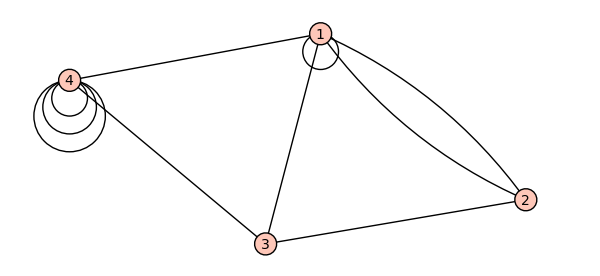
\includegraphics[width=10cm]{notes8-0.png}
\end{center}
For example, the graph pictured above would have the following matrix, where $m^i_j$ indicates the number of edges between the vertices labeled $i$~and~$j$:

\[
M = \begin{pmatrix}
1 & 2 & 1 & 1 \\
2 & 0 & 1 & 0 \\
1 & 1 & 0 & 1 \\
1 & 0 & 1 & 3 \\
\end{pmatrix}
\]
This is an example of a \emph{symmetric matrix}, since $m_j^i = m_i^j$.

\Videoscriptlink{matrices_example.mp4}{Adjacency Matrix Example}{scripts_matrices_example}
\end{example}

The set of all $r\times k$ matrices 
\[{\mathbb M}_k^r:=\{(m^i_j)|m^i_j\in {\mathbb R};\,  
i\in \{1,\dots,r\} ;\, 
j\in \{1\dots k\} \}\, ,\] 
is itself  a vector space with  addition and scalar multiplication defined as follows:

\Shabox{1}{\begin{tabular}{c}
$M+N = (m_j^i) + (n_j^i) = ( m_j^i + n_j^i )$\\[2mm]
$rM = r(m_j^i) = (rm_j^i)$\end{tabular}}

In other words, addition just adds corresponding entries in two matrices, and scalar multiplication multiplies every entry.
Notice that $M_1^n = \Re^n$ is just the vector space of column vectors.

Recall that we can multiply an \(r \times k\) matrix by a \(k \times 1\) column vector to produce a \(r \times 1\) column vector using the rule
\[MV = \big(\sum_{j=1}^k m_j^i v^j\big)\, .\]

This suggests the rule for multiplying an \(r \times k\) matrix \(M\) by a \(k \times s\) matrix~\(N\): our \(k \times s\) matrix \(N\) consists of \(s\) column vectors side-by-side, each of dimension \(k \times 1.\) We can multiply our \(r \times k\) matrix \(M\) by each of these \(s\) column vectors using the rule we already know, obtaining \(s\) column vectors each of dimension \(r \times 1.\) If we place these \(s\) column vectors side-by-side, we obtain an \(r \times s\) matrix \(MN.\)

That is, let \[N = 
\begin{pmatrix}
n_1^1 & n_2^1 & \cdots & n_s^1 \\
n_1^2 & n_2^2 & \cdots & n_s^2 \\
\multicolumn{1}{c}{\vdots} & \multicolumn{1}{c}{\vdots} &   & \multicolumn{1}{c}{\vdots} \\
n_1^k & n_2^k & \cdots & n_s^k \\
\end{pmatrix}
\]
and call the columns \(N_1\) through \(N_s\):
\[N_1 = \ccolvec{n_1^1\\n_1^2\\\vdots\\n_1^k}\, ,\:
N_2 = \ccolvec{n_2^1\\n_2^2\\\vdots\\n_2^k}\, ,\:
\ldots,\:
N_s = \ccolvec{n_s^1\\n_s^2\\\vdots\\n_s^k}.
\]
Then
%\[
%MN=M \rowvec{N_1 & N_2 & \cdots & N_s} = \rowvec{MN_1 & MN_2 & \cdots & MN_s}.
%\]
\[
MN=M
\begin{pmatrix}
\multicolumn{1}{c}{|} & \multicolumn{1}{c}{|} & & \multicolumn{1}{c}{|} \\
N_1 & N_2 & \cdots & N_s \\
\multicolumn{1}{c}{|} & \multicolumn{1}{c}{|} & & \multicolumn{1}{c}{|} \\
\end{pmatrix}
=
\begin{pmatrix}
\multicolumn{1}{c}{|} & \multicolumn{1}{c}{|} & & \multicolumn{1}{c}{|} \\
MN_1 & MN_2 & \cdots & MN_s \\
\multicolumn{1}{c}{|} & \multicolumn{1}{c}{|} & & \multicolumn{1}{c}{|} \\
\end{pmatrix}
\]

Concisely: If \(M=(m^i_j)\) for \(i=1, \ldots, r; j=1, \ldots, k\) and \(N=(n^i_j)\) for \(i=1, \ldots, k; j=1, \ldots, s,\) then \(MN=L\) where \(L=(\ell^i_j)\) for \(i=i, \ldots, r; j=1, \ldots, s\) is given by
\[
\ell^i_j = \sum_{p=1}^k m^i_p n^p_j.
\]
This rule obeys linearity.

Notice that in order for the multiplication to make sense, the columns and rows must match.  For an $r\times k$ matrix $M$ and an $s\times m$ matrix $N$, then to make the product $MN$ we must have $k=s$.  Likewise, for the product $NM$, it is required that $m=r$.  A common shorthand for keeping track of the sizes of the matrices involved in a given product is the following diagram.
\Shabox{1.05}{$\Big(r \times k\Big) { \text ~{\rm times}~} \Big(k\times m\Big) {\text ~{\rm is}~} \Big(r\times m\Big)$}

\Reading{Matrices}{2}


\begin{example}
Multiplying a $(3\times 1)$ matrix and a $(1\times 2)$ matrix yields a $(3\times 2)$ matrix.

\[
\colvec{1\\3\\2} \rowvec{2 & 3} = 
\begin{pmatrix}
1\cdot 2 & 1\cdot 3 \\
3\cdot 2 & 3\cdot 3 \\
2\cdot 2 & 2\cdot 3 \\
\end{pmatrix}
= \begin{pmatrix}
2 & 3 \\
6 & 9 \\
4 & 6 
\end{pmatrix} .
\]
\end{example}

Another way to view matrix multiplication is in terms of dot products:

\begin{center}
\shabox{The entries of $MN$ are made from the dot products of the rows of $M$ with the columns of $N$.}
\end{center}


\begin{example}
Let \[M=\begin{pmatrix}1&3\\3&5\\2&6\end{pmatrix}=:\ccolvec{u^T\\v^T\\w^T}
\mbox{ and }
N=\begin{pmatrix}2&3&1\\0&1&0\end{pmatrix}=:\rowvec{a & b & c}\]
where
\[
u=\colvec{1\\3}\, ,\quad
v=\colvec{3\\5}\, ,\quad 
w=\colvec{2\\6}\, ,\quad
a=\colvec{2\\0}\, ,\quad
b=\colvec{3\\1}\, ,\quad 
c=\colvec{1\\0}\, .
\]
Then 
\[
MN=\left(\!\begin{array}{ccc}
u\cdot a & u\cdot b & u\cdot c\\
v\cdot a & v\cdot b & v\cdot c\\
w\cdot a & w\cdot b & w\cdot c\\ 
\end{array}\!\right)
=
\begin{pmatrix}
2&6&1\\
6&14&3\\
4&12&2
\end{pmatrix}\, .
\]
\end{example}
This fact has an obvious yet important consequence:

\begin{theorem}
Let $M$ be a matrix and $x$ a column vector. If 
\[
Mx=0
\]
then the vector $x$ is \hyperlink{orthog}{orthogonal} to the rows of $M$.
\end{theorem}

\begin{remark}
Remember that the set of all vectors that can be obtained by adding up scalar multiples of the columns of a matrix is called its \hyperlink{column space}{column space}~\index{Column Space!concept of}. Similarly the {\bf row space}\index{Row Space} is the set of all row vectors obtained by adding up multiples of the rows of a matrix. The above theorem says that if $Mx=0$, then the vector $x$ is orthogonal to every vector in the row space of $M$.
\end{remark}


%\begin{center}\href{\webworkurl ReadingHomework8/1/}{Reading homework: problem 8.1}\end{center}

We know that $r\times k$ matrices can be used to represent linear transformations 
$ \Re^k \rightarrow \Re^r $
via \[(MV)^i = \sum_{j=1}^{k} m_j^iv^j , \] which is the same rule used when we multiply an $r\times k$ matrix by a $k\times 1$ vector to produce an $r\times1$ vector.

Likewise, we can use a matrix $N=(n^i_j)$ to define a linear transformation of a vector space of matrices. For example
\[
L \colon M^s_k \stackrel{N}{\longrightarrow} M^r_k\, ,
\]
\[
L(M)=(l^i_k) \mbox{ where } l^i_k= \sum_{j=1}^{s} n_j^im^j_k.
\]
This is the same as the rule we use to multiply matrices. \hypertarget{leftmult}{In other words,} \(L(M)=NM\) is a linear transformation.

\begin{definition}[Matrix Terminology]  
Let $M=(m^i_j)$ be a matrix. The entries $m_i^i$ are called {\bf diagonal}, and the set $\{m_1^1$, $m_2^2$, $\ldots \}$~is called the {\bf diagonal} of the matrix\index{Matrix!diagonal of}.

Any $r\times r$ matrix is called a {\bf square matrix}\index{Square matrix}.  A square matrix that is zero for all non-diagonal entries is called a {\bf diagonal matrix}\index{Diagonal matrix}. An example of a square diagonal matrix is
\[\begin{pmatrix}
2 & 0 & 0\\
0 & 3 & 0\\
0 & 0 & 0\\
\end{pmatrix}\, .\]

The $r\times r$ diagonal matrix with all diagonal entries equal to $1$ is called the {\bf identity matrix}\index{Identity matrix}, $I_r$, or just $I$.  An identity matrix looks like \[ I=
\begin{pmatrix}
1 & 0 & 0 & \cdots & 0 \\
0 & 1 & 0 & \cdots & 0 \\
0 & 0 & 1 & \cdots & 0 \\
\multicolumn{1}{c}{\vdots} & \multicolumn{1}{c}{\vdots} & \multicolumn{1}{c}{\vdots} & \ddots & \multicolumn{1}{c}{\vdots} \\
0 & 0 & 0 & \cdots & 1
\end{pmatrix}.
\]
The identity matrix is special because \[I_rM=MI_k=M\] for all $M$ of size $r\times k$.
\end{definition}



\begin{definition}
The {\bf transpose}\index{Transpose} of an $r\times k$ matrix $M = (m_j^i)$ is the $k\times r$ matrix 
\[
M^T = (\hat{m}_j^i)
\]
with entries that satisfy $\hat{m}_j^i = m_i^j$. \\

A matrix $M$ is \emph{symmetric}\index{Symmetric matrix} if $M=M^T$.
\end{definition}

\begin{example}
\[\begin{pmatrix}
2 & 5 & 6\\
1 & 3 & 4\\
\end{pmatrix}^T = 
\begin{pmatrix}
2 & 1 \\
5 & 3 \\
6 & 4 \\
\end{pmatrix}\, ,\]
and
\[
\begin{pmatrix}
2 & 5 & 6\\
1 & 3 & 4\\
\end{pmatrix}
\begin{pmatrix}
2 & 5 & 6\\
1 & 3 & 4\\
\end{pmatrix}^T = 
\begin{pmatrix}
65&43\\43&26
\end{pmatrix}\, ,\]
is symmetric.


\end{example}

%\begin{center}\href{\webworkurl ReadingHomework8/2/}{Reading homework: problem 8.2}\end{center}
\Reading{Matrices}{3}

\begin{remark}[Observations]

$\phantom{test}$

\begin{itemize}
\item Only square matrices can be symmetric.

\item The transpose of a column vector is a row vector, and vice-versa. 

\item Taking the transpose of a matrix twice does nothing.  \emph{i.e.,} $(M^T)^T=M$.
\end{itemize}
\end{remark}

\begin{theorem}[Transpose and Multiplication]
Let $M, N$ be matrices such that $MN$ makes sense.  Then 
\Shabox{1.05}{$(MN)^T = N^TM^T$.}
\end{theorem}
The proof of this theorem is left to \hyperref[MN=NTMT]{Review Question~\ref*{MN=NTMT}}.

%%%%%%%%%%%%%%%%%%%
\subsection{Associativity and Non-Commutativity }

Many properties of matrices following from the same property for real numbers. Here is an example.

\begin{example}
{\itshape Associativity of matrix multiplication.} We know for real numbers $x$, $y$ and $z$ that 
\[
x(yz)=(xy)z\, ,
\]
{\itshape i.e.}, the order of multiplications does not matter. The same property holds for matrix multiplication, let us show why.
Suppose $M=\big( m^i_j \big)$, $N=\big( n^j_k \big)$ and  $R=\big( r^k_l \big)$ are, 
respectively, $m\times n$, $n\times r$ and $r\times t$ matrices. Then from the rule for matrix
multiplication we have
\[
MN=\Big(\sum_{j=1}^n m^i_j n^j_k\Big)\mbox{ and } NR=\Big(\sum_{k=1}^r n^j_k r^k_l\Big)\, .
\]
So first we compute 
\[
(MN)R=\Big(\sum_{k=1}^r \Big[\sum_{j=1}^n m^i_j n^j_k\Big] r^k_l \Big) = 
\Big(\sum_{k=1}^r \sum_{j=1}^n \Big[ m^i_j n^j_k\Big] r^k_l \Big) =\Big(\sum_{k=1}^r \sum_{j=1}^n m^i_j n^j_k r^k_l \Big)\, .
\]
In the first step we just wrote out the definition for matrix multiplication, in the second step we
moved summation symbol outside the bracket (this is just the distributive
property $x(y+z)=xy+xz$ for numbers) and
in the last step we used the associativity property for real numbers to remove the square brackets. 
Exactly the same reasoning shows that
\[
M(NR)=\Big(\sum_{j=1}^n m^i_j\Big[\sum_{k=1}^r n^j_k r^k_l\Big]\Big) = 
\Big(\sum_{k=1}^r \sum_{j=1}^n  m^i_j \Big[n^j_kr^k_l \Big] \Big) =\Big(\sum_{k=1}^r \sum_{j=1}^n m^i_j n^j_k r^k_l \Big)\, .
\]
This is the same as above so we are done. \footnote{As a fun remark, note that Einstein would simply have written\\
$(MN)R=(m^i_j n^j_k) r^k_l= m^i_j n^j_k r^k_l = m^i_j (n^j_k r^k_l ) = M(NR)$.}
\end{example}
%%%%%%%%%%%%%% non-commute


Sometimes matrices do not share the properties of regular numbers. 
In particular, for {\itshape generic} $n\times n$ square matrices $M$ and $N$, 
\begin{center}
\shabox{\scalebox{1.1}{
$MN\neq NM\, .$ }}
\end{center}

\Videoscriptlink{matrices_commute.mp4}{Do Matrices Commute?}{script_matrices_commute}


\begin{example} (Matrix multiplication does \emph{not} commute.)
\[
\begin{pmatrix}
1 & 1 \\
0 & 1 \\
\end{pmatrix}
\begin{pmatrix}
1 & 0 \\
1 & 1 \\
\end{pmatrix} =
\begin{pmatrix}
2 & 1 \\
1 & 1 \\
\end{pmatrix}
\]
while, on the other hand,
\[
\begin{pmatrix}
1 & 0 \\
1 & 1 \\
\end{pmatrix}
\begin{pmatrix}
1 & 1 \\
0 & 1 \\
\end{pmatrix} =
\begin{pmatrix}
1 & 1 \\
1 & 2 \\
\end{pmatrix}\, .
\]
\end{example}
Since $n\times n$ matrices are linear transformations $\Re^n \rightarrow \Re^n$, we can see that the order of successive linear transformations matters.  
%In general  for two linear transformations $K$ and $L$ taking $\Re^n \rightarrow \Re^n$, and $v\in \Re^n$,  one has
%\[K(L(v)) \neq L(K(v))\, .\]
%Finding matrices such that $MN=NM$ is an important problem in mathematics.
%We promise

Here is an example of matrices acting on objects in three dimensions that also shows matrices not commuting.
\begin{example}
In \hyperlink{rotationprob}{Review Problem}~\ref{rotate}, you learned that the matrix
\[M=\begin{pmatrix}\cos\theta & \sin\theta \\ -\sin \theta & \cos\theta\end{pmatrix}\, ,\]
rotates vectors in the plane by an angle~$\theta$. 
We can generalize this, using \hyperlink{blocks}{block matrices}, to three dimensions.
In fact the following matrices built from a $2\times 2$ rotation matrix, a $1\times 1$ identity matrix and zeroes everywhere else
\[
M=\begin{pmatrix}\cos\theta & \sin\theta &0\\ -\sin \theta & \cos\theta&0\\\multicolumn{1}{c}{0}&\multicolumn{1}{c}{0}&1\end{pmatrix}\qquad\mbox{and}\qquad
N=\begin{pmatrix}1&\multicolumn{1}{c}{0}&\multicolumn{1}{c}{0}\\0&\cos\theta & \sin\theta \\ 0&-\sin \theta & \cos\theta\end{pmatrix}\, ,
\]
perform rotations by an angle $\theta$ in the $xy$ and $yz$ planes, respectively. Because, they rotate single vectors, you can also use them to rotate objects built from a collection of vectors like pretty colored blocks! Here is a picture of $M$ and then $N$ acting on such a block, compared with the case of $N$ followed by $M$. The special case of $\theta=90^\circ$ is shown.
\begin{center}
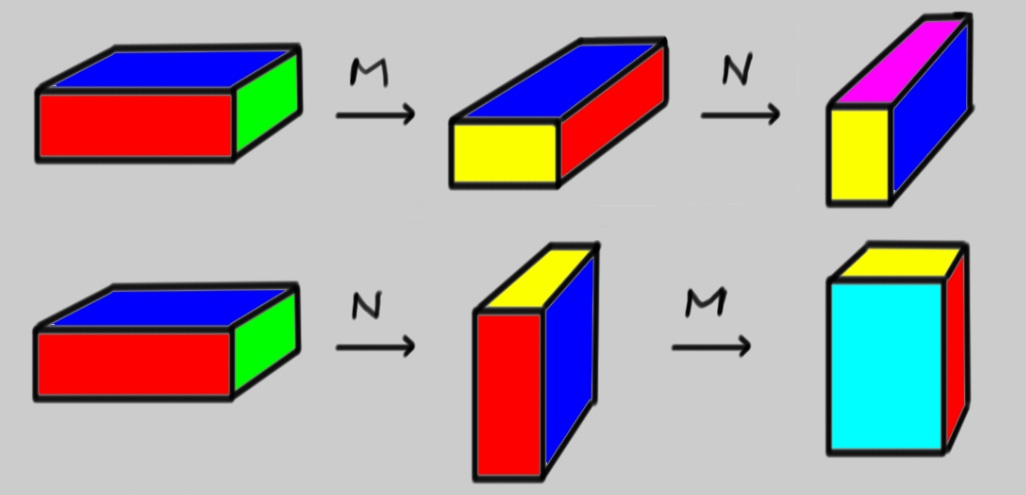
\includegraphics[scale=.3]{MNNM.jpg}
\end{center}
Notice how the endproducts of $MN$ and $NM$ are different, so $MN\neq NM$ here.
\end{example}



\subsection{Block Matrices}

It is often convenient to partition a matrix $M$ into smaller matrices called \hypertarget{blocks}{\emph{blocks}}. For example 

\[
M=\begin{pmat}{ccc|c}
1 & 2 & 3 & 1 \\
4 & 5 & 6 & 0 \\
7 & 8 & 9 & 1 \\
\cline{1-4}
0 & 1 & 2 & 0 \\
\end{pmat}
=
\begin{pmat}{c|c}
A & B \\
\cline{1-2}
C & D \\
\end{pmat}
\]
Where $A = \begin{pmatrix}
1 & 2 & 3 \\
4 & 5 & 6 \\
7 & 8 & 9 \\
\end{pmatrix}$, $B=\colvec{1\\0\\1}$, $C=\rowvec{0 & 1 & 2 }$, $D=(0)$.

\begin{itemize}
\item The blocks of a block matrix\index{Block matrix}  must fit together to form a rectangle.  So 
$\begin{pmat}{c|c}
B & A \\
\cline{1-2}
D & C \\
\end{pmat}
$ makes sense, but 
$\begin{pmat}{c|c}
C & B \\
\cline{1-2}
D & A \\
\end{pmat}
$ does not.

%\href{\webworkurl ReadingHomework9/1/}{Reading homework: problem 9.1}
\Reading{Matrices}{4}

\item There are many ways to cut up an $n\times n$ matrix into blocks.  Often context or the entries of the matrix will suggest a useful way to divide the matrix into blocks.  For example, if there are large blocks of zeros in a matrix, or blocks that look like an identity matrix, it can be useful to partition the matrix accordingly.

\item Matrix operations on block matrices can be carried out by treating the blocks as matrix entries.  In the example above,
\begin{eqnarray*}
M^2 & = & \begin{pmat}{c|c}
A & B \\
\cline{1-2}
C & D \\
\end{pmat}
\begin{pmat}{c|c}
A & B \\
\cline{1-2}
C & D \\
\end{pmat} \\[2mm]
& = & \begin{pmat}{c|c}
A^2+BC & AB+BD \\
\cline{1-2}
CA+DC & CB+D^2 \\
\end{pmat} \\
\end{eqnarray*}

Computing the individual blocks, we get:
\begin{eqnarray*}
A^2+BC &=& \begin{pmatrix}
	30 & 37 & 44 \\
	66 & 81 & 96 \\
	102&127 &152 \\
	\end{pmatrix} \\
AB+BD  &=& \colvec{ 4 \\ 10 \\ 16 } \\
CA+DC  &=& \rowvec{ 4 & 10 & 16 } \\
CB+D^2 &=& (2) 
\end{eqnarray*}

Assembling these pieces into a block matrix gives:
\[
\begin{pmat}{ccc|c}
30 & 37 & 44 & 4 \\
66 & 81 & 96 & 10 \\
102 & 127 & 152 & 16 \\
\cline{1-4}
4 & 10 & 16 & 2 \\
\end{pmat}
\]

This is exactly $M^2$.
\end{itemize}

\subsection{The Algebra of Square Matrices }\index{Square matrices}

Not every pair of matrices can be multiplied.  When multiplying two matrices, the number of rows in the left matrix must equal the number of columns in the right.  For an $r\times k$ matrix $M$ and an $s\times l$ matrix $N$, then we must have~$k=s$.

This is not a problem for square matrices of the same size, though.  Two~$n\times n$ matrices can be multiplied in either order.  For a single matrix $M \in \mathbb{M}^n_n$, we can form $M^2=MM$, $M^3=MMM$, and so on. It is useful to define \[M^0=I\, ,\] the identity matrix, just like $x^0=1$ for numbers.

As a result, any polynomial  can be have square matrices in it's domain. 

\begin{example}
Let $f(x) = x - 2x^2 + 3x^3$
and \[M=\begin{pmatrix}
1 & t \\
0 & 1 \\
\end{pmatrix}\, .\]  
Then 
\[
M^2 = \begin{pmatrix}
1 & 2t \\
0 & 1 \\
\end{pmatrix}\, ,\:\:
M^3 = \begin{pmatrix}
1 & 3t \\
0 & 1 \\
\end{pmatrix}\, ,\: \ldots
\]
and so 
\begin{eqnarray*}
f(M) &=& \begin{pmatrix}
	1 & t \\
	0 & 1 \\
	\end{pmatrix} 
- 2 \begin{pmatrix}
	1 & 2t \\
	0 & 1 \\
	\end{pmatrix} 
+ 3 \begin{pmatrix}
	1 & 3t \\
	0 & 1 \\
	\end{pmatrix} \\
&=& \begin{pmatrix}
	2 & 6t \\
	0 & 2 \\
	\end{pmatrix}.
\end{eqnarray*}
\end{example}

Suppose $f(x)$ is any function defined by a convergent Taylor Series:
\[
f(x) = f(0) + f'(0)x + \frac{1}{2!}f''(0)x^2 + \cdots\, .
\]
Then we can define the matrix function by just plugging in $M$:
\[
f(M) = f(0) + f'(0)M + \frac{1}{2!}f''(0)M^2 + \cdots\, .
\]
There are additional techniques to determine the convergence of Taylor Series of matrices, based on the fact that the convergence problem is simple for diagonal matrices.  It also turns out that the matrix exponential\index{Matrix exponential}
\[\exp (M) = I + M + \frac{1}{2}M^2 + \frac{1}{3!}M^3 + \cdots\, ,\] always converges.

\Videoscriptlink{properties_of_matrices_example.mp4}{Matrix Exponential Example}{properties_of_matrices_example}


\subsection{Trace}\index{Trace}

A large matrix contains a great deal of information, some of which often reflects the fact that you have not set up your problem efficiently. For example, a clever choice of basis can often make the matrix of a linear transformation very simple. Therefore, finding ways to extract the essential information of a matrix is useful. Here we need to assume that $n < \infty$ otherwise there are subtleties with convergence that we'd have to address.

\begin{definition}
The \hypertarget{TRACE}{{\bf trace}} of a square matrix $M=(m_j^i)$ is the sum of its diagonal entries:
\[
\tr M = \sum_{i=1}^{n}m_i^i\, .
\]
\end{definition}

\begin{example}
\[
\tr \begin{pmatrix}
2 & 7 & 6\\
9 & 5 & 1\\
4 & 3 & 8\\
\end{pmatrix} = 2+5+8 = 15\, .
\]
\end{example}
While matrix multiplication does not commute, the trace of a product of matrices does not depend on the order of multiplication:

\begin{eqnarray*}
\tr(MN) & = & \tr( \sum_l M_l^i N_j^l ) \\
& = & \sum_i \sum_l M_l^i N_i^l \\
& = & \sum_l \sum_i N_i^l M_l^i \\
& = & \tr( \sum_i N_i^l M_l^i ) \\
& = & \tr( NM ).
\end{eqnarray*}
\Videoscriptlink{properties_of_matrices_trace_proof.mp4}{Proof Explanation}{scripts_properties_of_matrices_trace_proof}
Thus we have a Theorem:
\begin{theorem} For any square matrices $M$ and $N$ \[\tr(MN)=\tr(NM).\]
\end{theorem}

\begin{example}
Continuing from the previous example, 

\[
M= \begin{pmatrix}
1 & 1 \\
0 & 1 \\
\end{pmatrix}, N=
\begin{pmatrix}
1 & 0 \\
1 & 1 \\
\end{pmatrix}.
\]
so
\[
MN = \begin{pmatrix}
2 & 1 \\
1 & 1 \\
\end{pmatrix} \neq
NM = \begin{pmatrix}
1 & 1 \\
1 & 2 \\
\end{pmatrix}.
\]
However, $\tr(MN) = 2+1 = 3 = 1+2 = \tr(NM)$.
\end{example}

Another useful property of the trace is that:
\[\tr M = \tr M^T\] 
This is true because the trace only uses the diagonal entries, which are fixed by the transpose.  For example, 
\[\tr \begin{pmatrix}
1 & 1 \\
2 & 3 \\
\end{pmatrix} = 4 = \tr \begin{pmatrix}
1 & 2 \\
1 & 3 \\
\end{pmatrix} = \tr \begin{pmatrix}
1 & 2 \\
1 & 3 \\
\end{pmatrix}^T\, .
\]
Finally, trace is a linear transformation from matrices to the real numbers.  This is easy to check.

%\Videoscriptlink{properties_of_matrices_trace.mp4}{More on the trace function}{scripts_properties_of_matrices_trace}

%\begin{remark}[Linear Systems Redux]
%
%Recall that we can view a linear system as a matrix equation
%\[MX=V,\] 
%with $M$ an $r\times k$ matrix of coefficients, $X$ a $k\times 1$ matrix of unknowns, and $V$ an $r\times 1$ matrix of constants.  If $M$ is a square matrix, then the number of equations~$r$ is the same as the number of unknowns~$k$, so we have hope of finding a single solution.
%
%Above we discussed functions of matrices.  An extremely useful function would be $f(M)=\frac{1}{M}$, where $M\frac{1}{M}=I$.  If we could compute $\frac{1}{M}$, then we would multiply both sides of the equation $MX=V$ by $\frac{1}{M}$ to obtain the solution immediately: $X=\frac{1}{M}V$.
%
%Clearly, if the linear system has no solution, then there can be no hope of finding $\frac{1}{M}$, since if it existed we could find a solution.  On the other hand, if the system has more than one solution, it also seems unlikely that $\frac{1}{M}$ would exist, since $X=\frac{1}{M}V$ yields only a single solution.  
%
%Therefore $\frac{1}{M}$ only sometimes exists.  It is called the \emph{inverse}\index{Inverse matrix!concept of} of $M$, and is usually written $M^{-1}$.
%\end{remark}
%

%\section*{References}
%Beezer: Part T, Section T
%\\
%Wikipedia:
%\begin{itemize}
%\item \href{http://en.wikipedia.org/wiki/Trace_(linear_algebra)}{Trace (Linear Algebra)}
%\item \href{http://en.wikipedia.org/wiki/Block_matrix}{Block Matrix}
%\end{itemize}
%

\section{Review Problems}

{\bf Webwork:} 
\begin{tabular}{|c|c|}
\hline
Reading Problems & \hwrref{Matrices}{2}, \hwrref{Matrices}{3},
 \hwrref{Matrices}{4}\\\hline
\end{tabular}





\begin{enumerate}
\item \label{det33} Let $M=\begin{pmatrix}
m^1_1 & m^1_2 & m^1_3\\
m^2_1 & m^2_2 & m^2_3\\
m^3_1 & m^3_2 & m^3_3\\
\end{pmatrix}$.  Use row operations to put $M$ into \emph{row echelon form}.  For simplicity, assume that $m_1^1\neq 0 \neq m^1_1m^2_2-m^2_1m^1_2$.

Prove that $M$ is non-singular if and only if:
\[
m^1_1m^2_2m^3_3 
- m^1_1m^2_3m^3_2 
+ m^1_2m^2_3m^3_1 
- m^1_2m^2_1m^3_3 
+ m^1_3m^2_1m^3_2
- m^1_3m^2_2m^3_1
\neq 0
\]

\phantomnewpage

\item 
\begin{enumerate}
\item What does the matrix $E^1_2=\begin{pmatrix}
0 & 1 \\
1 & 0
\end{pmatrix}$ do to $M=\begin{pmatrix}
a & b \\
d & c
\end{pmatrix}$ under left multiplication?  What about right multiplication?
\item Find elementary matrices $R^1(\lambda)$ and $R^2(\lambda)$ that respectively multiply rows $1$ and $2$ of $M$ by $\lambda$ but otherwise leave $M$ the same under left multiplication.
\item Find a matrix $S^1_2(\lambda)$ that adds a multiple $\lambda$ of row $2$ to row $1$ under left multiplication.
\end{enumerate}

\phantomnewpage

\item Let $M$ be a matrix and $S^i_jM$ the same matrix with rows \(i\) and \(j\) switched.  Explain every line of the 
\hyperlink{rowswap}{series of equations} proving that $\det M = -\det (S^i_jM)$.

\phantomnewpage

%\item \label{prob_inversion_number} This problem is a ``hands-on'' look at why \hyperlink{permutation_parity}{the property} describing the parity of permutations is true.
%
%\hypertarget{inversion_number}{The \emph{inversion number}}\index{Permutation!Inversion number} of a permutation $\sigma$ is the number of pairs $i<j$ such that $\sigma(i)>\sigma(j)$; it's the number of ``numbers that appear left of smaller numbers'' in the permutation.  For example, for the permutation $\rho = [4,2,3,1]$, the inversion number is $5$. The number $4$ comes before $2,3,$ and $1$, and $2$ and $3$ both come before $1$.
%
%Given a permutation $\sigma$, we can make a new permutation $\tau_{i,j} \sigma$ by exchanging the $i$th and $j$th entries of $\sigma$.
%
%\begin{enumerate}
%\item What is the inversion number of the permutation \(\mu=[1,2,4,3]\) that exchanges 4 and 3 and leaves everything else alone? Is it an even or an odd permutation?
%
%\item What is the inversion number of the permutation \(\rho=[4,2,3,1]\) that exchanges 1 and 4 and leaves everything else alone? Is it an even or an odd permutation?
%
%\item What is the inversion number of the permutation \(\tau_{1,3} \mu\)? Compare the parity\footnote{The \emph{parity} of an integer refers to whether the integer is even or odd. Here the parity of a permutation $\mu$ refers to the parity of its inversion number.} of \(\mu\) to the parity of \(\tau_{1,3} \mu.\)
%
%\item What is the inversion number of the permutation \(\tau_{2,4} \rho\)? Compare the parity of \(\rho\) to the parity of \(\tau_{2,4} \rho.\)
%
%\item What is the inversion number of the permutation \(\tau_{3,4} \rho\)? Compare the parity of \(\rho\) to the parity of \(\tau_{3,4} \rho.\)
%\end{enumerate}
%
%\videoscriptlink{elementary_matrices_determinant_hint.mp4}{Problem~\ref{prob_inversion_number} hints}{scripts_elementary_matrices_determinants_hint}

\phantomnewpage

%\item \label{problem_permutation} (Extra credit) Here we will examine a (very) small set of the general properties about permutations and their applications. In particular, we will show that one way to compute the sign of a permutation is by finding the \hyperlink{inversion_number}{inversion number} $N$ of $\sigma$ and we have
%\[
%\sgn(\sigma) = (-1)^N.
%\]
%
%For this problem, let $\mu = [1,2,4,3]$.
%
%\begin{enumerate}
%\item Show that every permutation $\sigma$ can be sorted by only taking simple (adjacent) transpositions\index{Permutation!Simple transposition} $s_i$ where $s_i$ interchanges the numbers in position $i$ and $i+1$ of a permutation $\sigma$ (in our other notation $s_i = \tau_{i,i+1}$). For example $s_2 \mu = [1, 4, 2, 3]$, and to sort $\mu$ we have $s_3 \mu = [1, 2, 3, 4]$.
%
%\item \label{prob_part_relations} We can compose simple transpositions together to represent a permutation (note that the sequence of compositions is not unique), and these are associative, we have an identity (the trivial permutation where the list is in order or we do nothing on our list), and we have an inverse since it is clear that $s_i s_i \sigma = \sigma$. Thus permutations of $[n]$ under composition are an example of a \hyperref[groups]{group}. However note that not all simple transpositions commute with each other since
%\begin{align*}
%s_1 s_2 [1, 2, 3] & = s_1 [1, 3, 2] = [3, 1, 2]
%\\ s_2 s_1 [1, 2, 3] & = s_2 [2, 1, 3] = [2, 3, 1]
%\end{align*}
%(you will prove here when simple transpositions commute). When we consider our initial permutation to be the trivial permutation $e = [1, 2, \dotsc, n]$, we do not write it; for example $s_i \equiv s_i e$ and $\mu = s_3 \equiv s_3 e$. This is analogous to not writing 1 when multiplying. Show that $s_i s_i = e$ (in shorthand $s_i^2 = e$), $s_{i+1} s_i s_{i+1} = s_i s_{i+1} s_i$ for all $i$, and $s_i$ and $s_j$ commute for all $|i - j| \geq 2$.
%
%\item Show that every way of expressing $\sigma$ can be obtained from using the relations proved in part~\ref{prob_part_relations}. In other words, show that for any expression $w$ of simple transpositions representing the trivial permutation $e$, using the proved relations.
%
%\emph{Hint: Use induction on $n$. For the induction step, follow the path of the $(n+1)$-th strand by looking at $s_n s_{n-1} \cdots s_k s_{k\pm1} \cdots s_n$ and argue why you can write this as a subexpression for any expression of $e$. Consider using diagrams of these paths to help.}
%
%\item The simple transpositions \hyperlink{action}{acts on} an $n$-dimensional vector space $V$ by $s_i v = E^i_{i+1} v$ (where $E^i_j$ is \hyperlink{elem_matrix_row_swap}{an elementary matrix}) for all vectors $v \in V$. Therefore we can just represent a permutation $\sigma$ as the matrix $M_{\sigma}$\footnote{Often people will just use $\sigma$ for the matrix when the context is clear.}, and we have $\det(M_{s_i}) = \det(E^i_{i+1}) = -1$. Thus prove that $\det(M_{\sigma}) = (-1)^N$ where $N$ is a number of simple transpositions needed to represent $\sigma$ as a permutation. You can assume that $M_{s_i s_j} = M_{s_i} M_{s_j}$ (it is not hard to prove) and that $\det(A B) = \det(A) \det(B)$ \hyperref[detmultiplicative]{from Chapter~\ref*{elementarydeterminantsII}}.
%
%\emph{Hint: You to make sure $\det(M_{\sigma})$ is well-defined since there are infinite ways to represent $\sigma$ as simple transpositions.}
%
%\item Show that $s_{i+1} s_i s_{i+1} = \tau_{i, i+2}$, and so give one way of writing $\tau_{i, j}$ in terms of simple transpositions? Is $\tau_{i,j}$ an even or an odd permutation? What is $\det(M_{\tau_{i,j}})$? What is the inversion number of $\tau_{i,j}$?
%
%\item The minimal number of simple transpositions needed to express $\sigma$ is called the \emph{length}\index{Permutation!Length} of $\sigma$; for example the length of $\mu$ is 1 since $\mu = s_3$. Show that the length of $\sigma$ is equal to the inversion number of $\sigma$.
%
%\emph{Hint: Find an procedure which gives you a new permutation $\sigma^{\prime}$ where $\sigma = s_i \sigma^{\prime}$ for some $i$ and the inversion number for $\sigma^{\prime}$ is 1 less than the inversion number for $\sigma$.}
%
%\item Show that $(-1)^N = \sgn(\sigma) = \det(M_{\sigma})$, where $\sigma$ is a permutation with $N$ inversions. Note that this immediately implies that $\sgn(\sigma \rho) = \sgn(\sigma) \sgn(\rho)$ for any permutations $\sigma$ and $\rho$.
%\end{enumerate}

\item Let $M'$ be the matrix obtained from $M$ by swapping two columns $i$ and $j$. Show that $\det M'=-\det M $.

\item The scalar triple product of three vectors $u,v,w$ from $\Re^3$ is $u\cdot(v\times w)$. Show that this product is the same as the determinant of the matrix whose columns are $u,v,w$ (in that order). What happens to the scalar triple product when the factors are permuted? 

\item Show that if $M$ is a $3\times 3$ matrix whose third row is a sum of multiples of the other rows ($R_3=aR_2+bR_1$) then $\det M=0$. Show that the same is true if one of the columns is a sum of multiples of the others. 

\end{enumerate}

\phantomnewpage

\section{\inverseMatTitle}
\label{inverse_matrix}


\begin{definition}
A square matrix $M$ is {\bf invertible} (or {\bf nonsingular})\index{Invertible}\index{Nonsingular} if there exists a matrix $M^{-1}$ such that
\[
M^{-1}M=I=MM^{-1}.
\]
If $M$ has no inverse, we say $M$ is {\bf singular}\index{singular} or {\bf non-invertible}\index{Non-invertible}.
\end{definition}

%\begin{figure}
%\begin{center}
%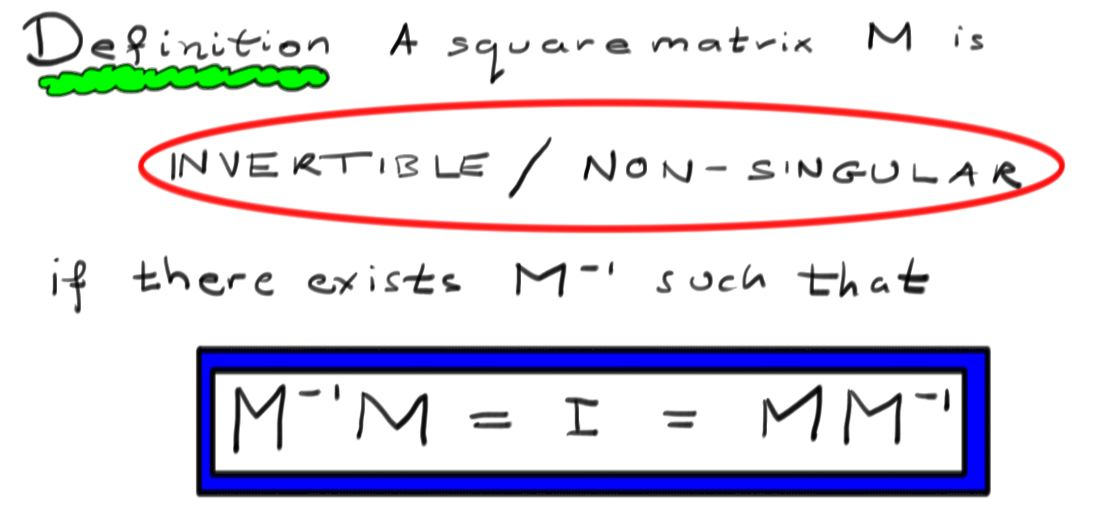
\includegraphics[scale=.27]{\inverseMatPath/defn_inverse_matrix.jpg}
%\end{center}
%\end{figure}


\begin{remark}[Inverse of a $2\times 2$ Matrix] Let $M$ and $N$ be the matrices:
\[
M=\begin{pmatrix}
a & b \\
c & d \\
\end{pmatrix},\qquad N=\begin{pmatrix}
d & -b \\
-c & a \\
\end{pmatrix}
\]
Multiplying these matrices gives:
\[
MN=\begin{pmatrix}
ad-bc & 0 \\
0 & ad-bc \\
\end{pmatrix}=(ad-bc)I\, .
\]
Then $M^{-1}=\frac{1}{ad-bc}\begin{pmatrix}
d & -b \\
-c & a \\
\end{pmatrix}$, so long as $ad-bc\neq 0$.    
\end{remark}

\begin{figure}
\begin{center}
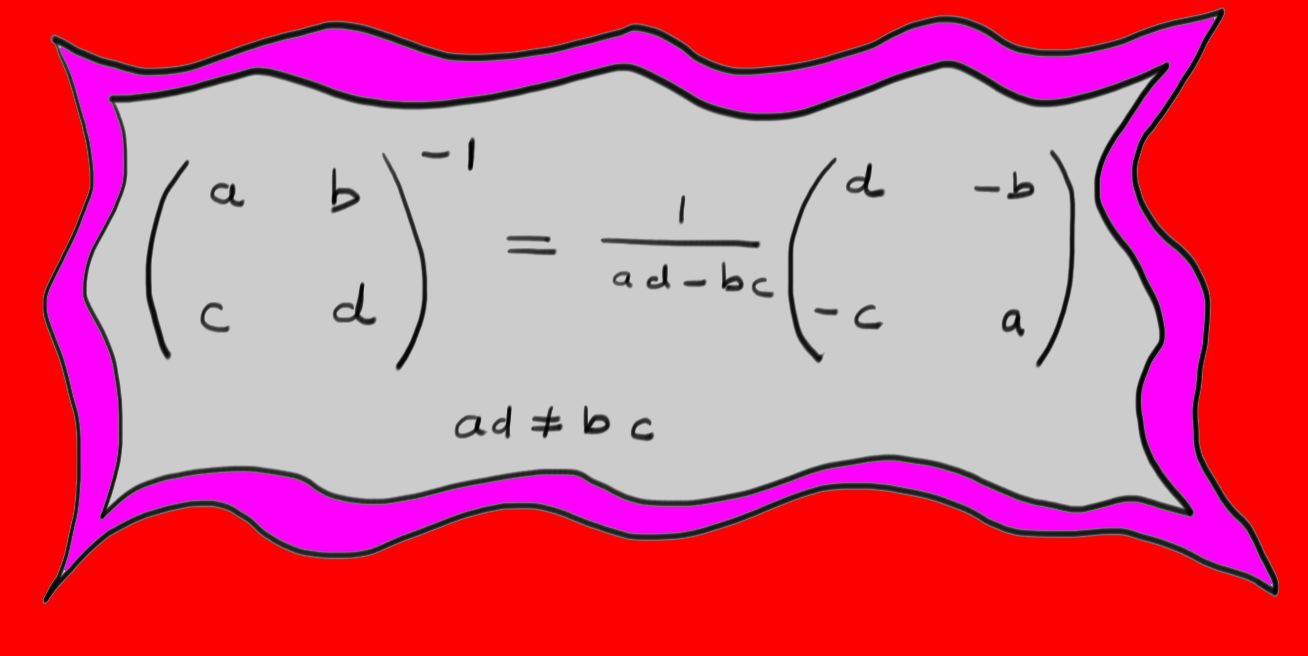
\includegraphics[scale=.24]{\inverseMatPath/2x2_inverse.jpg}
\end{center}
\caption{The formula for the inverse of a 2$\times$2 matrix is worth memorizing!}
\end{figure}



\subsection{Three Properties of the Inverse}

\begin{enumerate}
\item If $A$ is a square matrix and $B$ is the inverse of $A$, then $A$ is the inverse of $B$, since $AB=I=BA$.  So we have the identity
\[
(A^{-1})^{-1}=A.
\]

\item Notice that $B^{-1}A^{-1}AB=B^{-1}IB=I=ABB^{-1}A^{-1}$ so
\Shabox{1}{$
(AB)^{-1}=B^{-1}A^{-1}
$}
Thus, much like the transpose, taking the inverse of a product \emph{reverses} the order of the product.


%\begin{center}
%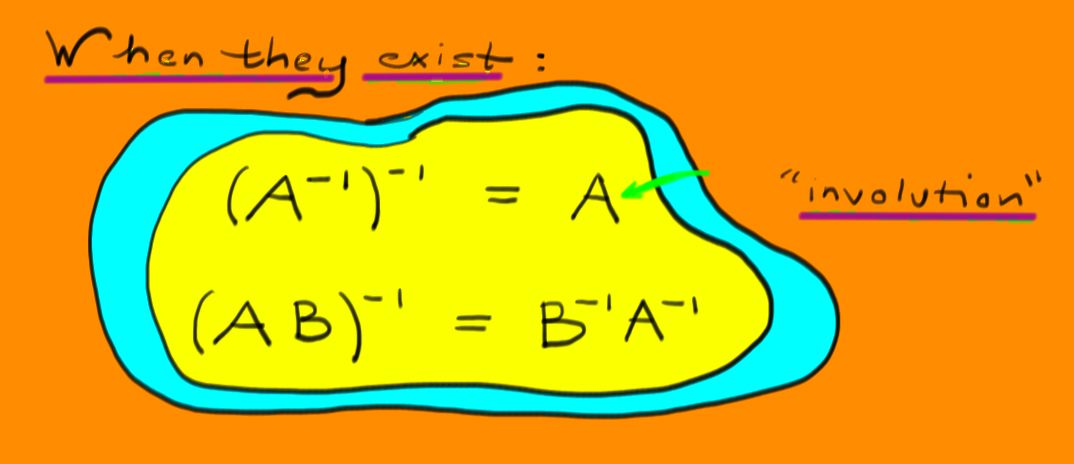
\includegraphics[scale=.26]{\inverseMatPath/inverse_inverse.jpg}
%\end{center}

\item Finally, recall that $(AB)^T=B^TA^T$.  Since $I^T=I$, then $(A^{-1}A)^T=A^T(A^{-1})^T=I$.  Similarly, $(AA^{-1})^T=(A^{-1})^TA^T=I$.  Then:
\[
(A^{-1})^T=(A^T)^{-1}
\]
%As such, we could even write $A^{-T}$ for the inverse of the transpose of $A$ (or equivalently the transpose of the inverse).
%\begin{center}
%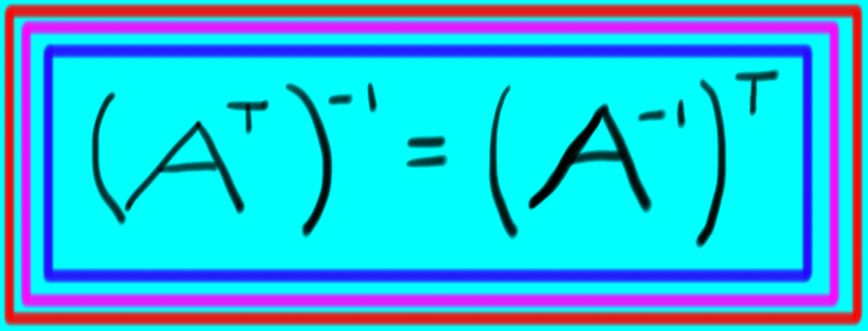
\includegraphics[scale=.20]{\inverseMatPath/transpose_inverse.jpg}
%\end{center}
\end{enumerate}

\Videoscriptlink{inverse_matrix_2by2_example.mp4}{$2\times 2$ Example}{scripts_inverse_matrix_2by2_example}




\subsection{Finding Inverses (Redux)}

Gaussian elimination can be used to find inverse matrices. This concept is covered in chapter~\ref{systems}, section~\ref{EROinverse},
but is presented here again as review in more sophisticated terms.


Suppose $M$ is a square invertible matrix and $MX=V$ is a linear system. The   solution
must be unique because it can be found by multiplying the equation on both sides by $M^{-1}$
yielding
 $X=M^{-1}V$. Thus,
the reduced row echelon form of the linear system has an identity matrix on the left:
\[
\begin{amatrix}{1}
M & V
\end{amatrix}
\sim
\begin{amatrix}{1}
I & M^{-1}V
\end{amatrix}
\]
Solving the linear system $MX=V$ then tells us what $M^{-1}V$ is.  

To solve many linear systems with the same matrix at once, 
\[MX=V_1,~MX=V_2\]
we can consider augmented matrices with 
%a matrix on the right side instead of a column vector, 
many columns on the right 
 and then apply Gaussian row reduction to the left side of the matrix.  Once the identity matrix is on the left side of the augmented matrix, then the solution of each of the individual linear systems is on the right.
 \[
\left(\begin{array}{c|cc}
\!M & V_1&V_2\!
\end{array}\right)
\sim
\left(\begin{array}{c|cc}
\!I & M^{-1}V_1 & M^{-1}V_2\!
\end{array}\right)
\]


To compute $M^{-1}$, we would like $M^{-1}$, rather than $M^{-1}V$ to appear on the right side of our augmented matrix.
This is achieved by  solving the collection of systems $MX=e_k$, where $e_k$ is the column vector of zeroes with a $1$ in the $k$th entry.  
{\itshape I.e.,} the $n\times n$ identity matrix can be viewed as a bunch of column vectors $I_n=(e_1 \ e_2 \ \cdots e_n)$. So, putting the $e_k$'s together into an identity matrix, we get:
\[
\begin{amatrix}{1}
M & I
\end{amatrix}
\sim
\begin{amatrix}{1}
I & M^{-1}I
\end{amatrix}
=\begin{amatrix}{1}
I & M^{-1}
\end{amatrix}
\]


\begin{example}
Find $\begin{pmatrix}
-1 & 2 & -3 \\
2 & 1 & 0 \\
4 & -2 & 5 \\
\end{pmatrix}^{-1}
$.

\noindent
We start by writing the augmented matrix, then apply row reduction to the left side.

\begin{eqnarray*}
\begin{pmat}{rrr|ccc}
-1 & 2 & -3 & 1 & 0 & 0 \\[1mm]
2  & 1 &  0 & 0 & 1 & 0 \\[1mm]
 4 & -2 & 5 & 0 & 0 & 1 \\[1mm]
\end{pmat} & \sim & \begin{pmat}{crr|ccc}
1  & -2&  3  & 1 & 0 & 0 \\[1mm]
0  & 5 &  -6 & 2 & 1 & 0 \\[1mm]
 0 & 6 & -7  & 4 & 0 & 1 \\[1mm]
\end{pmat} \\[2mm]
& \sim & \begin{pmat}{ccr|rrc}
1  & 0 &  \frac{3}{5}  & -\frac{1}{4} & \frac{2}{5} & 0 \\[1mm]
0  & 1 &  -\frac{6}{5} & \frac{2}{5} & \frac{1}{5}  & 0 \\[1mm]
 0 & 0 &  \frac{1}{5}  & \frac{4}{5} & -\frac{6}{5} & 1 \\[1mm]
\end{pmat} \\[2mm]
& \sim & \begin{pmat}{ccc|rrr}
1  & 0 &  0  & -5 & 4 & -3 \\[1mm]
0  & 1 &  0  & 10 & -7 & 6 \\[1mm]
 0 & 0 &  1  & 8 & -6 & 5 \\[1mm]
\end{pmat} \\
\end{eqnarray*}
At this point, we know $M^{-1}$ assuming we didn't goof up\index{Goofing up}.  However, row reduction is a lengthy and  involved process with lots of room for arithmetic errors, so we should~\emph{check our answer,} by confirming that $MM^{-1}=I$ (or if you prefer $M^{-1}M=I$):
\[MM^{-1} = 
\begin{pmatrix}
-1 & 2 & -3 \\
2 & 1 & 0 \\
4 & -2 & 5 \\
\end{pmatrix}\begin{pmatrix}
-5 & 4 & -3 \\
10 & -7 & 6 \\
 8 & -6 & 5 \\
\end{pmatrix}
=\begin{pmatrix}
1 & 0 & 0 \\
0 & 1 & 0 \\
0 & 0 & 1 \\
\end{pmatrix}
\]  
The product of the two matrices is indeed the identity matrix, so we're done.
\end{example}

%\href{\webworkurl ReadingHomework10/1/}{Reading homework: problem 10.1}
\Reading{Matrices}{5}
\subsection{Linear Systems and Inverses}

If $M^{-1}$ exists and is known, then we can immediately solve linear systems associated to $M$.

\begin{example}
Consider the linear system:

\[
      \begin{linsys}{2}
            -x & +2y & -3z         &=& 1  \\[1mm]
            2x & +\ y\,   &             &=& 2 \\[1mm]
            4x & -2y & +5z         &=& 0  
      \end{linsys}
\]
The associated matrix equation is $MX=\colvec{1\\2\\0},$ where \(M\) is the same as in the previous section, so the system above is equivalent to the matrix equation

\[
\colvec{x\\y\\z}=\begin{pmatrix}
-1 & 2 & -3 \\
2 & 1 & 0 \\
4 & -2 & 5 \\
\end{pmatrix}^{-1}\colvec{1\\2\\0}
=\begin{pmatrix}
-5 & 4 & -3 \\
10 & -7 & 6 \\
 8 & -6 & 5 \\
\end{pmatrix}\colvec{1\\2\\0}
=\colvec{3\\-4\\-4}.
\]
That is, the system is equivalent to the equation $\colvec{x\\y\\z}=\colvec{3\\-4\\-4}$, and it is easy to see what the solution(s) to this equation are. 
\end{example}
In summary, when $M^{-1}$ exists 

\begin{center}
\shabox{$Mx=v \Leftrightarrow x=M^{-1}v\, .$}
\end{center}


%\href{\webworkurl ReadingHomework10/2/}{Reading homework: problem 10.2}
\Reading{Matrices}{5}

\subsection{Homogeneous Systems}

\begin{theorem}
A square matrix $M$ is invertible if and only if the homogeneous system \[Mx=0\] has no non-zero solutions.
\end{theorem}

\begin{proof}
First, suppose that $M^{-1}$ exists.  Then $Mx=0 \Rightarrow x=M^{-1}0=0$.  Thus, if $M$ is invertible, then $Mx=0$ has no non-zero solutions.

On the other hand, $Mx=0$ always has the solution $x=0$.  If no other solutions exist, then $M$ can be put into reduced row echelon form with every variable a pivot.  In this case, $M^{-1}$ can be computed using the process in the previous section.
\end{proof}

%\begin{figure}
\begin{center}
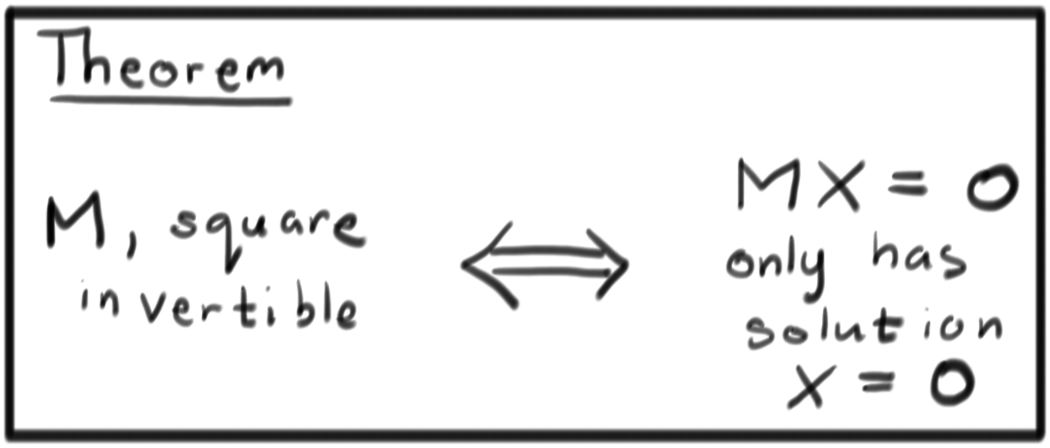
\includegraphics[scale=.26]{\inverseMatPath/inverse_theorem.jpg}
\end{center}
%\end{figure}

%A great test of your linear algebra knowledge is to make a list of conditions for a matrix to be singular.
%You will learn more of these as the course goes by, but can also skip straight to the list in Section~\ref{thelist}. 

\subsection{Bit Matrices}\index{Bit matrices}
In computer science, information is recorded using binary strings of data.  For example, the following string contains an English word:
\[
011011000110100101101110011001010110000101110010
\]
A \hypertarget{bits}{\emph{bit}} is the basic unit of information, keeping track of a single one or zero.  Computers can add and multiply individual bits very quickly.

In chapter~\ref{vectorSpaces}, section~\ref{otherfields} it is explained how to formulate vector spaces over \hyperref[fields]{fields} other than real numbers.
In particular, al of the properties of a 
vector space make sense with numbers $\Z_2=\{0,1 \}$ with addition and multiplication given by the following tables. 
\label{Z2}
\[
\begin{array}{c|cc}
+ & 0 & 1 \\ \hline
0 & 0 & 1 \\
1 & 1 & 0 \\
\end{array}
\qquad
\begin{array}{c|cc}
\times& 0 & 1 \\ \hline
0 & 0 & 0 \\
1 & 0 & 1 \\
\end{array}
\]
Notice that $-1=1$, since $1+1=0$.
Therefore,  we can apply all of the linear algebra we have learned thus far to matrices with $\Z_2$ entries.  A matrix with entries in $\Z_2$ is sometimes called a \emph{bit matrix}\index{Bit Matrix}.

\begin{example}
$\begin{pmatrix}
1 & 0 & 1 \\
0 & 1 & 1 \\
1 & 1 & 1 \\
\end{pmatrix}$ is an invertible matrix over $\Z_2$;

\[\begin{pmatrix}
1 & 0 & 1 \\
0 & 1 & 1 \\
1 & 1 & 1 \\
\end{pmatrix}^{-1}=\begin{pmatrix}
0 & 1 & 1 \\
1 & 0 & 1 \\
1 & 1 & 1 \\
\end{pmatrix}.
\]

This can be easily verified by multiplying:

\[\begin{pmatrix}
1 & 0 & 1 \\
0 & 1 & 1 \\
1 & 1 & 1 \\
\end{pmatrix}\begin{pmatrix}
0 & 1 & 1 \\
1 & 0 & 1 \\
1 & 1 & 1 \\
\end{pmatrix}=\begin{pmatrix}
1 & 0 & 0 \\
0 & 1 & 0 \\
0 & 0 & 1 \\
\end{pmatrix}
\]
\end{example}

\begin{remark}[Application: Cryptography]  
A very simple way to hide information is to use a substitution cipher, in which the alphabet is permuted and each letter in a message is systematically exchanged for another.  For example, the ROT-13 cypher just exchanges a letter with the letter thirteen places before or after it in the alphabet.  For example, HELLO becomes URYYB.  Applying the algorithm again decodes the message, turning URYYB back into HELLO.  Substitution ciphers are easy to break, but the basic idea can be extended to create cryptographic systems that are practically uncrackable.  For example, a \emph{one-time pad} is a system that uses a different substitution for each letter in the message.  So long as a particular set of substitutions is not used on more than one message, the one-time pad is unbreakable.

English characters are often stored in computers in the ASCII format.  In ASCII, a single character is represented by a string of eight bits, which we can consider as a vector in $\Z_2^8$ (which is like vectors in $\Re^8$, where the entries are zeros and ones).  One way to create a substitution cipher, then, is to choose an $8\times 8$ invertible bit matrix $M$, and multiply each letter of the message by $M$.  Then to decode the message, each string of eight characters would be multiplied by $M^{-1}$.  

To make the message a bit tougher to decode, one could consider pairs (or longer sequences) of letters as a single vector in $\Z_2^{16}$ (or a higher-dimensional space), and then use an appropriately-sized invertible matrix.
For more on cryptography, see ``The Code Book,'' by Simon Singh (1999, Doubleday).
\end{remark}

%{\itshape You should now be ready to attempt the \hyperref[sample1]{first sample midterm}.}
%\begin{center}
%\shabox{
%\begin{tabular}{c}
%\itshape \hyperref[sample1]{You are now ready to attempt the first sample midterm}. 
%\\
%\hyperref[sample1]{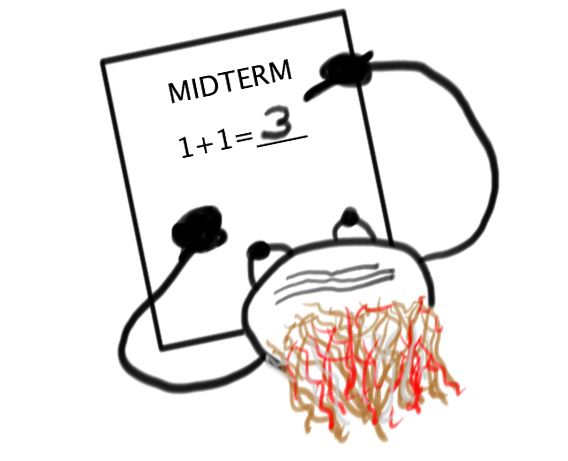
\includegraphics[scale=.15]{midterm.jpg}}
%\end{tabular}
%}
%\end{center}
%
%\section*{References}
%
%Hefferon: Chapter Three, Section IV.2
%\\
%Beezer: Chapter M, Section MISLE
%\\
%Wikipedia:
%\href{http://en.wikipedia.org/wiki/Invertible_matrix}{Invertible Matrix}
%
%
\section{Review Problems}
{\bf Webwork:} 
\begin{tabular}{|c|c|}
\hline
Reading Problems & \hwrref{Matrices}{6}, \hwrref{Matrices}{7}
 \\
 \hline
\end{tabular}






\begin{enumerate}
\item \label{det33} Let $M=\begin{pmatrix}
m^1_1 & m^1_2 & m^1_3\\
m^2_1 & m^2_2 & m^2_3\\
m^3_1 & m^3_2 & m^3_3\\
\end{pmatrix}$.  Use row operations to put $M$ into \emph{row echelon form}.  For simplicity, assume that $m_1^1\neq 0 \neq m^1_1m^2_2-m^2_1m^1_2$.

Prove that $M$ is non-singular if and only if:
\[
m^1_1m^2_2m^3_3 
- m^1_1m^2_3m^3_2 
+ m^1_2m^2_3m^3_1 
- m^1_2m^2_1m^3_3 
+ m^1_3m^2_1m^3_2
- m^1_3m^2_2m^3_1
\neq 0
\]

\phantomnewpage

\item 
\begin{enumerate}
\item What does the matrix $E^1_2=\begin{pmatrix}
0 & 1 \\
1 & 0
\end{pmatrix}$ do to $M=\begin{pmatrix}
a & b \\
d & c
\end{pmatrix}$ under left multiplication?  What about right multiplication?
\item Find elementary matrices $R^1(\lambda)$ and $R^2(\lambda)$ that respectively multiply rows $1$ and $2$ of $M$ by $\lambda$ but otherwise leave $M$ the same under left multiplication.
\item Find a matrix $S^1_2(\lambda)$ that adds a multiple $\lambda$ of row $2$ to row $1$ under left multiplication.
\end{enumerate}

\phantomnewpage

\item Let $M$ be a matrix and $S^i_jM$ the same matrix with rows \(i\) and \(j\) switched.  Explain every line of the 
\hyperlink{rowswap}{series of equations} proving that $\det M = -\det (S^i_jM)$.

\phantomnewpage

%\item \label{prob_inversion_number} This problem is a ``hands-on'' look at why \hyperlink{permutation_parity}{the property} describing the parity of permutations is true.
%
%\hypertarget{inversion_number}{The \emph{inversion number}}\index{Permutation!Inversion number} of a permutation $\sigma$ is the number of pairs $i<j$ such that $\sigma(i)>\sigma(j)$; it's the number of ``numbers that appear left of smaller numbers'' in the permutation.  For example, for the permutation $\rho = [4,2,3,1]$, the inversion number is $5$. The number $4$ comes before $2,3,$ and $1$, and $2$ and $3$ both come before $1$.
%
%Given a permutation $\sigma$, we can make a new permutation $\tau_{i,j} \sigma$ by exchanging the $i$th and $j$th entries of $\sigma$.
%
%\begin{enumerate}
%\item What is the inversion number of the permutation \(\mu=[1,2,4,3]\) that exchanges 4 and 3 and leaves everything else alone? Is it an even or an odd permutation?
%
%\item What is the inversion number of the permutation \(\rho=[4,2,3,1]\) that exchanges 1 and 4 and leaves everything else alone? Is it an even or an odd permutation?
%
%\item What is the inversion number of the permutation \(\tau_{1,3} \mu\)? Compare the parity\footnote{The \emph{parity} of an integer refers to whether the integer is even or odd. Here the parity of a permutation $\mu$ refers to the parity of its inversion number.} of \(\mu\) to the parity of \(\tau_{1,3} \mu.\)
%
%\item What is the inversion number of the permutation \(\tau_{2,4} \rho\)? Compare the parity of \(\rho\) to the parity of \(\tau_{2,4} \rho.\)
%
%\item What is the inversion number of the permutation \(\tau_{3,4} \rho\)? Compare the parity of \(\rho\) to the parity of \(\tau_{3,4} \rho.\)
%\end{enumerate}
%
%\videoscriptlink{elementary_matrices_determinant_hint.mp4}{Problem~\ref{prob_inversion_number} hints}{scripts_elementary_matrices_determinants_hint}

\phantomnewpage

%\item \label{problem_permutation} (Extra credit) Here we will examine a (very) small set of the general properties about permutations and their applications. In particular, we will show that one way to compute the sign of a permutation is by finding the \hyperlink{inversion_number}{inversion number} $N$ of $\sigma$ and we have
%\[
%\sgn(\sigma) = (-1)^N.
%\]
%
%For this problem, let $\mu = [1,2,4,3]$.
%
%\begin{enumerate}
%\item Show that every permutation $\sigma$ can be sorted by only taking simple (adjacent) transpositions\index{Permutation!Simple transposition} $s_i$ where $s_i$ interchanges the numbers in position $i$ and $i+1$ of a permutation $\sigma$ (in our other notation $s_i = \tau_{i,i+1}$). For example $s_2 \mu = [1, 4, 2, 3]$, and to sort $\mu$ we have $s_3 \mu = [1, 2, 3, 4]$.
%
%\item \label{prob_part_relations} We can compose simple transpositions together to represent a permutation (note that the sequence of compositions is not unique), and these are associative, we have an identity (the trivial permutation where the list is in order or we do nothing on our list), and we have an inverse since it is clear that $s_i s_i \sigma = \sigma$. Thus permutations of $[n]$ under composition are an example of a \hyperref[groups]{group}. However note that not all simple transpositions commute with each other since
%\begin{align*}
%s_1 s_2 [1, 2, 3] & = s_1 [1, 3, 2] = [3, 1, 2]
%\\ s_2 s_1 [1, 2, 3] & = s_2 [2, 1, 3] = [2, 3, 1]
%\end{align*}
%(you will prove here when simple transpositions commute). When we consider our initial permutation to be the trivial permutation $e = [1, 2, \dotsc, n]$, we do not write it; for example $s_i \equiv s_i e$ and $\mu = s_3 \equiv s_3 e$. This is analogous to not writing 1 when multiplying. Show that $s_i s_i = e$ (in shorthand $s_i^2 = e$), $s_{i+1} s_i s_{i+1} = s_i s_{i+1} s_i$ for all $i$, and $s_i$ and $s_j$ commute for all $|i - j| \geq 2$.
%
%\item Show that every way of expressing $\sigma$ can be obtained from using the relations proved in part~\ref{prob_part_relations}. In other words, show that for any expression $w$ of simple transpositions representing the trivial permutation $e$, using the proved relations.
%
%\emph{Hint: Use induction on $n$. For the induction step, follow the path of the $(n+1)$-th strand by looking at $s_n s_{n-1} \cdots s_k s_{k\pm1} \cdots s_n$ and argue why you can write this as a subexpression for any expression of $e$. Consider using diagrams of these paths to help.}
%
%\item The simple transpositions \hyperlink{action}{acts on} an $n$-dimensional vector space $V$ by $s_i v = E^i_{i+1} v$ (where $E^i_j$ is \hyperlink{elem_matrix_row_swap}{an elementary matrix}) for all vectors $v \in V$. Therefore we can just represent a permutation $\sigma$ as the matrix $M_{\sigma}$\footnote{Often people will just use $\sigma$ for the matrix when the context is clear.}, and we have $\det(M_{s_i}) = \det(E^i_{i+1}) = -1$. Thus prove that $\det(M_{\sigma}) = (-1)^N$ where $N$ is a number of simple transpositions needed to represent $\sigma$ as a permutation. You can assume that $M_{s_i s_j} = M_{s_i} M_{s_j}$ (it is not hard to prove) and that $\det(A B) = \det(A) \det(B)$ \hyperref[detmultiplicative]{from Chapter~\ref*{elementarydeterminantsII}}.
%
%\emph{Hint: You to make sure $\det(M_{\sigma})$ is well-defined since there are infinite ways to represent $\sigma$ as simple transpositions.}
%
%\item Show that $s_{i+1} s_i s_{i+1} = \tau_{i, i+2}$, and so give one way of writing $\tau_{i, j}$ in terms of simple transpositions? Is $\tau_{i,j}$ an even or an odd permutation? What is $\det(M_{\tau_{i,j}})$? What is the inversion number of $\tau_{i,j}$?
%
%\item The minimal number of simple transpositions needed to express $\sigma$ is called the \emph{length}\index{Permutation!Length} of $\sigma$; for example the length of $\mu$ is 1 since $\mu = s_3$. Show that the length of $\sigma$ is equal to the inversion number of $\sigma$.
%
%\emph{Hint: Find an procedure which gives you a new permutation $\sigma^{\prime}$ where $\sigma = s_i \sigma^{\prime}$ for some $i$ and the inversion number for $\sigma^{\prime}$ is 1 less than the inversion number for $\sigma$.}
%
%\item Show that $(-1)^N = \sgn(\sigma) = \det(M_{\sigma})$, where $\sigma$ is a permutation with $N$ inversions. Note that this immediately implies that $\sgn(\sigma \rho) = \sgn(\sigma) \sgn(\rho)$ for any permutations $\sigma$ and $\rho$.
%\end{enumerate}

\item Let $M'$ be the matrix obtained from $M$ by swapping two columns $i$ and $j$. Show that $\det M'=-\det M $.

\item The scalar triple product of three vectors $u,v,w$ from $\Re^3$ is $u\cdot(v\times w)$. Show that this product is the same as the determinant of the matrix whose columns are $u,v,w$ (in that order). What happens to the scalar triple product when the factors are permuted? 

\item Show that if $M$ is a $3\times 3$ matrix whose third row is a sum of multiples of the other rows ($R_3=aR_2+bR_1$) then $\det M=0$. Show that the same is true if one of the columns is a sum of multiples of the others. 

\end{enumerate}

\phantomnewpage

\newpage

\section{LU Redux}
\label{LUdecomp}

Certain matrices are easier to work with than others.  In this section, we will see how to write any square\footnote{The case where $M$ is not square is dealt with at the end of the section.} matrix $M$ as the product of two simpler matrices.  We will write \[M=LU\, ,\] where:
\begin{itemize}
\item $L$ is \emph{lower triangular}\index{Lower triangular matrix}.  This means that all entries above the main diagonal are zero.  In notation,
$L=(l^i_j)$ with $l^i_j=0$ for all $j>i$.
\[L=\begin{pmatrix}
l^1_1 & 0 & 0 & \cdots \\
l^2_1 & l^2_2 & 0 & \cdots \\
l^3_1 & l^3_2 & l^3_3 & \cdots \\
\vdots & \vdots & \vdots & \ddots \\
\end{pmatrix}
\]

\item $U$ is \emph{upper triangular}\index{Upper triangular matrix}.  This means that all entries below the main diagonal are zero.  In notation,
$U=(u^i_j)$ with $u^i_j=0$ for all $j<i$.
\[U=\begin{pmatrix}
u^1_1 & u^1_2 & u^1_3 & \cdots \\
0 & u^2_2 & u^2_3 & \cdots \\
0 & 0 & u^3_3 & \cdots \\
\vdots & \vdots & \vdots & \ddots \\
\end{pmatrix}
\]
\end{itemize}
$M=LU$ is called an \emph{$LU$ decomposition}\index{LU@$LU$ decomposition} of $M$.

This is a useful trick for  computational reasons; it is much easier to compute the inverse of an upper or lower triangular matrix than general matrices.  Since inverses are useful for solving linear systems, this makes solving any linear system associated to the matrix much faster as well.  The determinant---a very important quantity associated with any square matrix---is very easy to compute for triangular matrices.

\begin{example}
Linear systems associated to upper triangular matrices are very easy to solve by back substitution.
\[
\begin{amatrix}{2}
a & b & 1 \\
0 & c & e \\
\end{amatrix} \ \Rightarrow \ y=\frac{e}{c}\, , \quad x=\frac{1}{a}\left(1-\frac{be}{c}\right)
\]

\[
\begin{amatrix}{3}
1 & 0 & 0 & d \\
a & 1 & 0 & e \\
b & c & 1 & f \\
\end{amatrix} 
\Rightarrow 
\left\{    \begin{array}{l} x=d\\   y=e-ax\\  z=f-bx-cy \end{array} \right\}
\Rightarrow 
\left\{    \begin{array}{l} x=d\\   y=e-ad\\  z=f-bd-c(e-ad) \end{array} \right. .
\]
For lower triangular matrices, 
\emph{forward} substitution\index{Forward substitution} 
gives a quick solution; for upper triangular matrices, 
\emph{back} substitution\index{Back substitution} 
gives the solution.
\end{example}





\subsection{Using $LU$ Decomposition to Solve Linear Systems}

Suppose we have $M=LU$ and want to solve the system
\[
MX=LUX=V.
\]

\begin{itemize}
\item{Step 1:} Set $W=\colvec{u\\v\\w}=UX$.  

\item{Step 2:} Solve the system $LW=V$.  This should be simple by forward substitution since $L$ is lower triangular.  Suppose the solution to $LW=V$ is $W_0$.  

\item{Step 3:} Now solve the system $UX=W_0$.  This should be easy by backward substitution, since $U$ is upper triangular.  The solution to this system is the solution to the original system.
\end{itemize}
We can think of this as using the matrix $L$ to perform row operations on the matrix $U$ in order to solve the system; this idea also appears in the  study of determinants.

%\href{\webworkurl ReadingHomework11/1/}{Reading homework: problem 11.1}
\Reading{Matrices}{7}

\begin{example}
Consider the linear system:
\[
      \begin{linsys}{4}
            6x & +&18y & +&3z         &=& 3  \\[1mm]
            2x & +&12y & +&z	    &=& 19 \\[1mm]
            4x & +&15y & +&3z         &=& 0  
      \end{linsys}
\]

An $LU$ decomposition for the associated matrix $M$ is
\[
\begin{pmatrix}
6 & 18 & 3 \\
2 & 12 & 1 \\
4 & 15 & 3 
\end{pmatrix} =
\begin{pmatrix}
3 & 0 & 0 \\
1 & 6 & 0 \\
2 & 3 & 1 
\end{pmatrix}
\begin{pmatrix}
2 & 6 & 1 \\
0 & 1 & 0 \\
0 & 0 & 1 
\end{pmatrix}.
\]

\begin{itemize}
\item{Step 1:} \hypertarget{LUproc}{Set} $W=\colvec{u\\v\\w}=UX$.  

\item{Step 2:} Solve the system $LW=V$:

\[
\begin{pmatrix}
3 & 0 & 0 \\
1 & 6 & 0 \\
2 & 3 & 1 
\end{pmatrix}
\colvec{u\\v\\w} =
\colvec{3\\19\\0}
\]

By substitution, we get $u=1$, $v=3$, and $w=-11$.  Then 
\[W_0=\colvec{1\\3\\-11}\]

\item{Step 3:} Solve the system $UX=W_0$.  
\[
\begin{pmatrix}
2 & 6 & 1 \\
0 & 1 & 0 \\
0 & 0 & 1 
\end{pmatrix}
\colvec{x\\y\\z} =
\colvec{1\\3\\-11}
\]
Back substitution gives $z=-11, y=3$, and $x=-3$.  

Then $X=\colvec{-3\\3\\-11}$, and we're done.
\end{itemize}
\end{example}

\Videoscriptlink{lu_decomposition_using_lu_decomp.mp4}{Using an $LU$ decomposition}{scripts_lu_decomposition_using_lu_example}

%\begin{figure}
\begin{center}
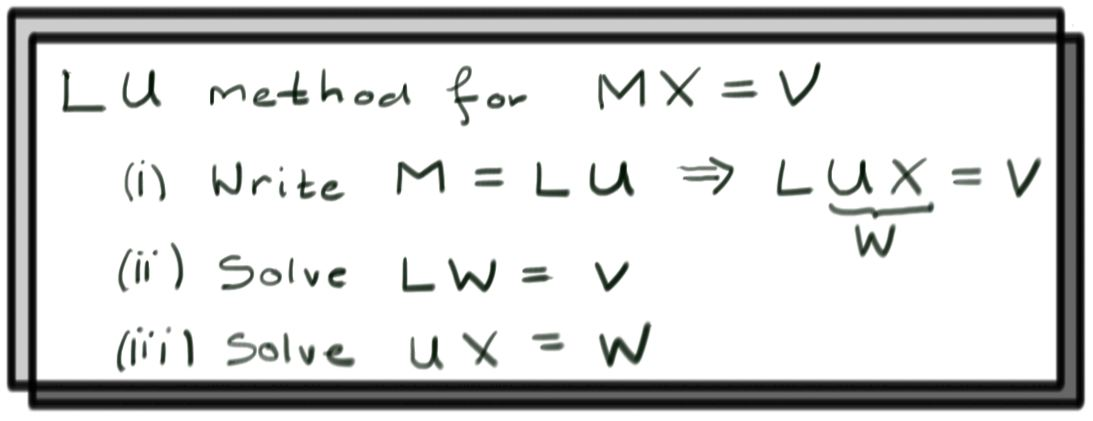
\includegraphics[scale=.3]{\luDecompPath/LU_solution.jpg}
\end{center}
%\end{figure}

\subsection{Finding an $LU$ Decomposition.}
\label{finding_LU_decomp}

In chapter~\ref{systems}, section~\ref{LUtake1}, Gaussian elimination was used to find~$LU$ matrix decompositions.  
These ideas are presented here again as review.
 
For any given matrix, there are actually many different $LU$ decompositions.  However, there is a unique $LU$ decomposition in which the $L$ matrix has ones on the diagonal. In that case $L$ is called a \emph{lower unit triangular matrix}\index{Lower unit triangular matrix}.

To find the $LU$ decomposition, we'll create two sequences of matrices $L_1, L_2,\ldots$ and $U_1, U_2, \ldots$ such that at each step, $L_iU_i=M$.  Each of the $L_i$ will be lower triangular, but only the last $U_i$ will be upper triangular.
 The main trick for this calculation is captured by the following example:

\begin{example} (An Elementary Matrix)

\noindent
Consider \[E=\begin{pmatrix}1&0\\\lambda&1\end{pmatrix}\, ,\qquad M=\begin{pmatrix}a&b&c&\cdots\\d&e&f&\cdots\end{pmatrix}\, .\]
Lets compute $EM$
\[
EM=\begin{pmatrix}\multicolumn{1}{c}{a}&\mc{b}&\mc{c}&\cdots\\d+\lambda a&e+\lambda b&f+\lambda c&\cdots\end{pmatrix}\, .
\]
Something neat happened here: multiplying $M$ by $E$ performed the row operation $R_2\to R_2+\lambda R_1$ on $M$.
Another interesting fact:
\[
E^{-1}:=\begin{pmatrix}1&0\\-\lambda&1\end{pmatrix}
\] 
obeys (check this yourself...)
\[
E^{-1} E = 1\, .
\]
Hence $M=E^{-1} E M$ or, writing this out
\[
\begin{pmatrix}a&b&c&\cdots\\d&e&f&\cdots\end{pmatrix}=\begin{pmatrix}1&0\\-\lambda&1\end{pmatrix} \begin{pmatrix}\mc{a}&\mc{b}&\mc{c}&\cdots\\d+\lambda a&e+\lambda b&f+\lambda c&\cdots\end{pmatrix}\, .
\]
Here the matrix on the left is lower triangular, while the matrix on the right has had a row operation performed on it.
\end{example}




\vspace{2mm}
We would like to  use the first row of $M$ to zero out the first entry of every row below it.  For our running example, \[M=\begin{pmatrix}
6 & 18 & 3 \\
2 & 12 & 1 \\
4 & 15 & 3 
\end{pmatrix}\, ,\] so we would like to perform the row operations \[R_2\to R_2 -\frac 13 R_1 \mbox{ and } R_3\to R_3-\frac 23R_1\, .\]
%so the second row minus $\frac{1}{3}$ of the first row will zero out the first entry in the second row.  Likewise, the third row minus $\frac{2}{3}$ of the first row will zero out the first entry in the third row.
If we perform these row operations on $M$ to produce 
\[U_1=\begin{pmatrix}
6 & 18 & 3 \\
0 & 6 & 0 \\
0 & 3 & 1 
\end{pmatrix}\, ,\]
we need to multiply this on the left by a lower triangular matrix $L_1$ so that the product $L_1U_1=M$ still.
The above example shows how to do this:
Set $L_1$ to be the lower triangular matrix whose first column is filled with  {\bf minus} the constants used to zero out the first column of $M$.  Then \[L_1 = \begin{pmatrix}
1 & 0 & 0 \\[1mm]
\frac{1}{3} & 1 & 0 \\[1mm]
\frac{2}{3} & 0 & 1 
\end{pmatrix}\, .\]  
%Set $U_1$ to be the matrix obtained by zeroing out the first column of $M$.  Then $U_1=\begin{pmatrix}
%6 & 18 & 3 \\
%0 & 6 & 0 \\
%0 & 3 & 1 
%\end{pmatrix}$.
By construction $L_1 U_1=M$, but you should compute this yourself as a double check.

Now repeat the process by zeroing the second column of $U_1$ below the diagonal using the second row of $U_1$ using the row operation
$R_3\to R_3-\frac 12 R_2$ to produce
\[U_2=\begin{pmatrix}6&18&3\\0&6&0\\0&0&1\end{pmatrix}\, .\]
The matrix that undoes this row operation is obtained in the same way we found $L_1$ above and is:
\[
\begin{pmatrix}
1&0&0\\
0&1&0\\
0&\frac 12& 1
\end{pmatrix}\, .
\]
Thus our answer for $L_2$ is the product of this matrix with $L_1$, namely
\[
L_2=
\begin{pmatrix}
1 & 0 & 0 \\[1mm]
\frac{1}{3} & 1 & 0 \\[1mm]
\frac{2}{3} & 0 & 1 
\end{pmatrix}\begin{pmatrix}
1&0&0\\
0&1&0\\
0&\frac 12& 1
\end{pmatrix}
=\begin{pmatrix}
1 & 0 & 0 \\[1mm]
\frac{1}{3} & 1 & 0 \\[1mm]
\frac{2}{3} & \frac{1}{2} & 1 
\end{pmatrix}\, .
\]
Notice that it is lower triangular because 

\begin{center}
\shabox{The product of lower triangular matrices is always lower triangular!}
\end{center}

\noindent
Moreover it is obtained by recording minus the constants used for all our row operations in the appropriate columns (this always works this way).
Moreover, $U_2$ is upper triangular and $M=L_2U_2$, we are done!
Putting this all together we have
\[M=\begin{pmatrix}
6 & 18 & 3 \\
2 & 12 & 1 \\
4 & 15 & 3 
\end{pmatrix}= \begin{pmatrix}
1 & 0 & 0 \\[1mm]
\frac{1}{3} & 1 & 0 \\[1mm]
\frac{2}{3} & \frac{1}{2} & 1 
\end{pmatrix}\begin{pmatrix}
6 & 18 & 3 \\[1mm]
0 & 6 & 0 \\[1mm]
0 & 0 & 1 
\end{pmatrix}\, .\]  
%Since $U_2$ is upper-triangular, we're done.  Inserting the new number into $L_1$ to get $L_2$ really is safe: the numbers in the first column don't affect the second column of $U_1$, since the first column of $U_1$ is already zeroed out.

If the matrix you're working with has more than three rows, just continue this process by zeroing out the next column below the diagonal, and repeat until there's nothing left to do.

\Videoscriptlink{lu_decomposition_example.mp4}{Another $LU$ decomposition example}{scripts_lu_decomposition_example}

The fractions in the $L$ matrix are admittedly ugly.  For two matrices $LU$, we can multiply one entire column of $L$ by a constant $\lambda$ and divide the corresponding row of $U$ by the same constant without changing the product of the two matrices.  Then:

\begin{eqnarray*}
LU &=& \begin{pmatrix}
1 & 0 & 0 \\[1mm]
\frac{1}{3} & 1 & 0 \\[1mm]
\frac{2}{3} & \frac{1}{2} & 1 
\end{pmatrix}
I
\begin{pmatrix}
6 & 18 & 3 \\[1mm]
0 & 6 & 0 \\[1mm]
0 & 0 & 1 
\end{pmatrix} \\
&=&
\begin{pmatrix}
1 & 0 & 0 \\[1mm]
\frac{1}{3} & 1 & 0 \\[1mm]
\frac{2}{3} & \frac{1}{2} & 1 
\end{pmatrix}
\begin{pmatrix}
3 & 0 & 0 \\
0 & 6 & 0 \\
0 & 0 & 1 
\end{pmatrix}
\begin{pmatrix}
\frac{1}{3} & 0 & 0 \\[1mm]
0 & \frac{1}{6} & 0 \\[1mm]
0 & 0 & 1 
\end{pmatrix}
\begin{pmatrix}
6 & 18 & 3 \\
0 & 6 & 0 \\
0 & 0 & 1 
\end{pmatrix} \\
&=&
\begin{pmatrix}
3 & 0 & 0 \\
1 & 6 & 0 \\
2 & 3 & 1 
\end{pmatrix}\begin{pmatrix}
2 & 6 & 1 \\
0 & 1 & 0 \\
0 & 0 & 1 
\end{pmatrix}.
\end{eqnarray*}
The resulting matrix looks nicer, but isn't in standard (lower unit triangular matrix) form.

\Reading{Matrices}{7}
%\href{\webworkurl ReadingHomework11/2/}{Reading homework: problem 11.2}

For matrices that are not square, $LU$ decomposition still makes sense.  Given an $m\times n$ matrix $M$, for example we could write $M=LU$ with $L$ a square lower unit triangular matrix, and $U$ a rectangular matrix.  Then $L$ will be an $m\times m$ matrix, and $U$ will be an $m\times n$ matrix (of the same shape as $M$).  From here, the process is exactly the same as for a square matrix.  We create a sequence of matrices $L_i$ and $U_i$ that is eventually the $LU$ decomposition.  Again, we start with $L_0=I$ and $U_0=M$.

\begin{example}
Let's find the $LU$ decomposition of $M=U_0=\begin{pmatrix}
-2 & 1 & 3 \\
-4 & 4 & 1 
\end{pmatrix}$.  Since $M$ is a $2\times 3$ matrix, our decomposition will consist of a $2\times 2$ matrix and a $2\times 3$ matrix.  Then we start with $L_0=I_2=\begin{pmatrix}
1 & 0 \\
0 & 1
\end{pmatrix}$.

The next step is to zero-out the first column of $M$ below the diagonal.  There is only one row to cancel, then, and it can be removed by subtracting $2$ times the first row of $M$ to the second row of $M$.  Then:

\[
L_1=\begin{pmatrix}
1 & 0 \\
2 & 1
\end{pmatrix}, \qquad 
U_1 = \begin{pmatrix}
-2 & 1 & 3 \\
0 & 2 & -5 
\end{pmatrix}
\]
Since $U_1$ is upper triangular, we're done.  With a larger matrix, we would just continue the process.
\end{example}





\subsection{Block $LDU$ Decomposition}

Let $M$ be a square block matrix with square blocks $X,Y,Z,W$ such that $X^{-1}$ exists.  Then $M$ can be decomposed as a block $LDU$ decomposition, where $D$ is block diagonal, as follows:
\[
M=\begin{pmatrix}
X & Y \\
Z & W
\end{pmatrix}
\]
Then: 
\begin{center}
\shabox{
$M=\left(\begin{array}{cc}
I &  0 \\[1mm]
ZX^{-1} & I
\end{array}\right)
\left(\begin{array}{cc}
X & 0 \\[1mm]
0 & W-ZX^{-1}Y
\end{array}\right)\left(\begin{array}{cc}
I & X^{-1}Y \\[1mm]
0 & I
\end{array}\right)\, .$}\end{center}
This can be checked explicitly simply by block-multiplying these three matrices.

\Videoscriptlink{lu_decomposition_blocks.mp4}{Block $LDU$ Explanation}{scripts_lu_decomposition_blocks}

\begin{example}
For a $2\times 2$ matrix, we can regard each entry as a $1\times1$ block.
\[
\begin{pmatrix}
1 & 2 \\
3 & 4
\end{pmatrix}=
\begin{pmatrix}
1 & 0 \\
3 & 1
\end{pmatrix}
\begin{pmatrix}
1 & 0 \\
0 & -2
\end{pmatrix}
\begin{pmatrix}
1 & 2 \\
0 & 1
\end{pmatrix}
\]
By multiplying the diagonal matrix by the upper triangular matrix, we get the standard $LU$ decomposition of the matrix.
\end{example}


%{\bf You should now be ready to attempt the \hyperref[sample1]{first sample midterm}.}
\begin{center}
\shabox{
\begin{tabular}{c}
\bf \hyperref[sample1]{You are now ready to attempt the first sample midterm}. 
\\
\hyperref[sample1]{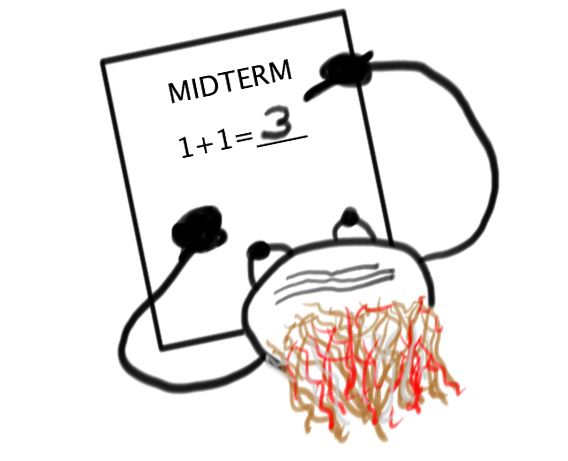
\includegraphics[scale=.15]{midterm.jpg}}
\end{tabular}
}
\end{center}

%\section*{References}
%Wikipedia:
%\begin{itemize}
%\item \href{http://en.wikipedia.org/wiki/LU_decomposition}{$LU$ Decomposition}
%\item \href{http://en.wikipedia.org/wiki/Block_LU_decomposition}{Block $LU$ Decomposition}
%\end{itemize}

\section{Review Problems}
{\bf Webwork:} 
\begin{tabular}{|c|c|}
\hline
Reading Problems & 
 \hwrref{Matrices}{7},\hwrref{Matrices}{8}\\
 $LU$ Decomposition & \hwref{Matrices}{14}\\
 \hline
\end{tabular}




\begin{enumerate}
\item \label{det33} Let $M=\begin{pmatrix}
m^1_1 & m^1_2 & m^1_3\\
m^2_1 & m^2_2 & m^2_3\\
m^3_1 & m^3_2 & m^3_3\\
\end{pmatrix}$.  Use row operations to put $M$ into \emph{row echelon form}.  For simplicity, assume that $m_1^1\neq 0 \neq m^1_1m^2_2-m^2_1m^1_2$.

Prove that $M$ is non-singular if and only if:
\[
m^1_1m^2_2m^3_3 
- m^1_1m^2_3m^3_2 
+ m^1_2m^2_3m^3_1 
- m^1_2m^2_1m^3_3 
+ m^1_3m^2_1m^3_2
- m^1_3m^2_2m^3_1
\neq 0
\]

\phantomnewpage

\item 
\begin{enumerate}
\item What does the matrix $E^1_2=\begin{pmatrix}
0 & 1 \\
1 & 0
\end{pmatrix}$ do to $M=\begin{pmatrix}
a & b \\
d & c
\end{pmatrix}$ under left multiplication?  What about right multiplication?
\item Find elementary matrices $R^1(\lambda)$ and $R^2(\lambda)$ that respectively multiply rows $1$ and $2$ of $M$ by $\lambda$ but otherwise leave $M$ the same under left multiplication.
\item Find a matrix $S^1_2(\lambda)$ that adds a multiple $\lambda$ of row $2$ to row $1$ under left multiplication.
\end{enumerate}

\phantomnewpage

\item Let $M$ be a matrix and $S^i_jM$ the same matrix with rows \(i\) and \(j\) switched.  Explain every line of the 
\hyperlink{rowswap}{series of equations} proving that $\det M = -\det (S^i_jM)$.

\phantomnewpage

%\item \label{prob_inversion_number} This problem is a ``hands-on'' look at why \hyperlink{permutation_parity}{the property} describing the parity of permutations is true.
%
%\hypertarget{inversion_number}{The \emph{inversion number}}\index{Permutation!Inversion number} of a permutation $\sigma$ is the number of pairs $i<j$ such that $\sigma(i)>\sigma(j)$; it's the number of ``numbers that appear left of smaller numbers'' in the permutation.  For example, for the permutation $\rho = [4,2,3,1]$, the inversion number is $5$. The number $4$ comes before $2,3,$ and $1$, and $2$ and $3$ both come before $1$.
%
%Given a permutation $\sigma$, we can make a new permutation $\tau_{i,j} \sigma$ by exchanging the $i$th and $j$th entries of $\sigma$.
%
%\begin{enumerate}
%\item What is the inversion number of the permutation \(\mu=[1,2,4,3]\) that exchanges 4 and 3 and leaves everything else alone? Is it an even or an odd permutation?
%
%\item What is the inversion number of the permutation \(\rho=[4,2,3,1]\) that exchanges 1 and 4 and leaves everything else alone? Is it an even or an odd permutation?
%
%\item What is the inversion number of the permutation \(\tau_{1,3} \mu\)? Compare the parity\footnote{The \emph{parity} of an integer refers to whether the integer is even or odd. Here the parity of a permutation $\mu$ refers to the parity of its inversion number.} of \(\mu\) to the parity of \(\tau_{1,3} \mu.\)
%
%\item What is the inversion number of the permutation \(\tau_{2,4} \rho\)? Compare the parity of \(\rho\) to the parity of \(\tau_{2,4} \rho.\)
%
%\item What is the inversion number of the permutation \(\tau_{3,4} \rho\)? Compare the parity of \(\rho\) to the parity of \(\tau_{3,4} \rho.\)
%\end{enumerate}
%
%\videoscriptlink{elementary_matrices_determinant_hint.mp4}{Problem~\ref{prob_inversion_number} hints}{scripts_elementary_matrices_determinants_hint}

\phantomnewpage

%\item \label{problem_permutation} (Extra credit) Here we will examine a (very) small set of the general properties about permutations and their applications. In particular, we will show that one way to compute the sign of a permutation is by finding the \hyperlink{inversion_number}{inversion number} $N$ of $\sigma$ and we have
%\[
%\sgn(\sigma) = (-1)^N.
%\]
%
%For this problem, let $\mu = [1,2,4,3]$.
%
%\begin{enumerate}
%\item Show that every permutation $\sigma$ can be sorted by only taking simple (adjacent) transpositions\index{Permutation!Simple transposition} $s_i$ where $s_i$ interchanges the numbers in position $i$ and $i+1$ of a permutation $\sigma$ (in our other notation $s_i = \tau_{i,i+1}$). For example $s_2 \mu = [1, 4, 2, 3]$, and to sort $\mu$ we have $s_3 \mu = [1, 2, 3, 4]$.
%
%\item \label{prob_part_relations} We can compose simple transpositions together to represent a permutation (note that the sequence of compositions is not unique), and these are associative, we have an identity (the trivial permutation where the list is in order or we do nothing on our list), and we have an inverse since it is clear that $s_i s_i \sigma = \sigma$. Thus permutations of $[n]$ under composition are an example of a \hyperref[groups]{group}. However note that not all simple transpositions commute with each other since
%\begin{align*}
%s_1 s_2 [1, 2, 3] & = s_1 [1, 3, 2] = [3, 1, 2]
%\\ s_2 s_1 [1, 2, 3] & = s_2 [2, 1, 3] = [2, 3, 1]
%\end{align*}
%(you will prove here when simple transpositions commute). When we consider our initial permutation to be the trivial permutation $e = [1, 2, \dotsc, n]$, we do not write it; for example $s_i \equiv s_i e$ and $\mu = s_3 \equiv s_3 e$. This is analogous to not writing 1 when multiplying. Show that $s_i s_i = e$ (in shorthand $s_i^2 = e$), $s_{i+1} s_i s_{i+1} = s_i s_{i+1} s_i$ for all $i$, and $s_i$ and $s_j$ commute for all $|i - j| \geq 2$.
%
%\item Show that every way of expressing $\sigma$ can be obtained from using the relations proved in part~\ref{prob_part_relations}. In other words, show that for any expression $w$ of simple transpositions representing the trivial permutation $e$, using the proved relations.
%
%\emph{Hint: Use induction on $n$. For the induction step, follow the path of the $(n+1)$-th strand by looking at $s_n s_{n-1} \cdots s_k s_{k\pm1} \cdots s_n$ and argue why you can write this as a subexpression for any expression of $e$. Consider using diagrams of these paths to help.}
%
%\item The simple transpositions \hyperlink{action}{acts on} an $n$-dimensional vector space $V$ by $s_i v = E^i_{i+1} v$ (where $E^i_j$ is \hyperlink{elem_matrix_row_swap}{an elementary matrix}) for all vectors $v \in V$. Therefore we can just represent a permutation $\sigma$ as the matrix $M_{\sigma}$\footnote{Often people will just use $\sigma$ for the matrix when the context is clear.}, and we have $\det(M_{s_i}) = \det(E^i_{i+1}) = -1$. Thus prove that $\det(M_{\sigma}) = (-1)^N$ where $N$ is a number of simple transpositions needed to represent $\sigma$ as a permutation. You can assume that $M_{s_i s_j} = M_{s_i} M_{s_j}$ (it is not hard to prove) and that $\det(A B) = \det(A) \det(B)$ \hyperref[detmultiplicative]{from Chapter~\ref*{elementarydeterminantsII}}.
%
%\emph{Hint: You to make sure $\det(M_{\sigma})$ is well-defined since there are infinite ways to represent $\sigma$ as simple transpositions.}
%
%\item Show that $s_{i+1} s_i s_{i+1} = \tau_{i, i+2}$, and so give one way of writing $\tau_{i, j}$ in terms of simple transpositions? Is $\tau_{i,j}$ an even or an odd permutation? What is $\det(M_{\tau_{i,j}})$? What is the inversion number of $\tau_{i,j}$?
%
%\item The minimal number of simple transpositions needed to express $\sigma$ is called the \emph{length}\index{Permutation!Length} of $\sigma$; for example the length of $\mu$ is 1 since $\mu = s_3$. Show that the length of $\sigma$ is equal to the inversion number of $\sigma$.
%
%\emph{Hint: Find an procedure which gives you a new permutation $\sigma^{\prime}$ where $\sigma = s_i \sigma^{\prime}$ for some $i$ and the inversion number for $\sigma^{\prime}$ is 1 less than the inversion number for $\sigma$.}
%
%\item Show that $(-1)^N = \sgn(\sigma) = \det(M_{\sigma})$, where $\sigma$ is a permutation with $N$ inversions. Note that this immediately implies that $\sgn(\sigma \rho) = \sgn(\sigma) \sgn(\rho)$ for any permutations $\sigma$ and $\rho$.
%\end{enumerate}

\item Let $M'$ be the matrix obtained from $M$ by swapping two columns $i$ and $j$. Show that $\det M'=-\det M $.

\item The scalar triple product of three vectors $u,v,w$ from $\Re^3$ is $u\cdot(v\times w)$. Show that this product is the same as the determinant of the matrix whose columns are $u,v,w$ (in that order). What happens to the scalar triple product when the factors are permuted? 

\item Show that if $M$ is a $3\times 3$ matrix whose third row is a sum of multiples of the other rows ($R_3=aR_2+bR_1$) then $\det M=0$. Show that the same is true if one of the columns is a sum of multiples of the others. 

\end{enumerate}

\phantomnewpage

\newpage




